% !TEX root = ../master_thesis.tex
\chapter{Préliminaires théoriques}\label{chap:théorie}

Dans ce chapitre, nous détaillons les fondements théoriques nécessaires à la compréhension de la spectroscopie Raman et des travaux de ce mémoire. Nous partons de l'Hamiltonien général d'un solide cristallin et des approximations qui permettent de découpler le problème en une partie électronique et une partie ionique. Nous verrons comment résoudre ces deux parties, introduirons les fonctions de Wannier et présenterons brièvement le couplage entre la lumière et les électrons du système. 

\section{Hamiltonien général d'un solide cristallin}\label{sec:H_général}

Toute l'information d'un système quantique est contenue dans la fonction d'onde $\Psi$ et sa connaissance nous donne accès à toutes les propriétés du système. Pour la trouver, il faut résoudre l'équation de Schrödinger
\begin{equation}
    \hat{H}\Psi = E\Psi,
\end{equation}
où $\hat{H}$ est l'opérateur qui représente l'énergie totale du système et $E$ est l'énergie totale. Les systèmes qui nous intéressent sont des solides cristallins composés d'atomes arrangés périodiquement sur un réseau cristallin. Ces atomes sont constitués d'électrons de valence, responsables des propriétés physiques et chimiques d'intérêt, et d'électrons de c\oe ur, fortement liés aux noyaux et chimiquement inertes. Ces derniers sont traités conjointement avec les noyaux pour former des ions de masses $M_{I}$ et de pseudo-charge $Z_{I}$. Tous ces constituants sont électriquement chargés et interagissent mutuellement par l'entremise d'un potentiel de Coulomb. L'Hamiltonien général qui représente un ensemble de $N_e$ électrons et $N_i$ ions est donné par
\begin{equation}
\begin{split}
    \hat{H} &= -\sum_{i=1}^{N_e}\frac{\hbar^2}{2m_e}\nabla_i^2
        -\sum_{I=1}^{N_i}\frac{\hbar^2}{2M_I}\nabla_I^2
        +\frac{1}{2}\sum_{\substack{IJ \\ I\neq J}}^{N_i}
        \frac{Z_IZ_Je^2}{4\pi\varepsilon_0|\rv_I-\rv_J|} \\
      &\quad +\frac{1}{2}\sum_{\substack{ij \\ i\neq j}}
        \frac{e^2}{4\pi\varepsilon_0|\rv_i-\rv_j|}+\sum_{i=1}^{N_e}V_\text{ext}(\rv_i),
\end{split}
\label{eqn:c2_H_general}
\end{equation}
où nous reconnaissons, dans l'ordre, l'énergie cinétique des électrons, l'énergie cinétique des ions, la répulsion Coulombienne ion-ion, la répulsion Coulombienne électron-électron et l'attraction Coulombienne électron-ion, encodée dans le potentiel externe $V_\text{ext}(\rv)$ qui sera remplacé par un pseudo-potentiel dans la section~\ref{sec:PP}. Dans ce mémoire, des termes supplémentaires à cet Hamiltonien seront introduits aux chapitres~\ref{chap:défauts} et~\ref{chap:eph} pour décrire le couplage des électrons avec les défauts dans le système et les vibrations des ions \textit{i.e.} les phonons.

Bien qu'il soit relativement facile de poser le problème, sa résolution l'est beaucoup moins. Nous faisons face ici à un problème à $N=N_e+N_i$ corps couplés par l'interaction Coulombienne, dont la fonction d'onde $\Psi(\{\rv_i\},\{\rv_I\})$ dépend simultanément de $3N$ variables. Le nombre de paramètres nécessaires pour représenter cette fonction d'onde croît exponentiellement avec le nombre de particules $N$ : pour un système de seulement 10 particules discrétisé sur une grille de $10\times10\times10=10^3$ points, il faudrait $(10^3)^{10}=10^{30}$ valeurs -- soit davantage que tout ce que l'humanité a jamais enregistré~\cite{hilbertWorldsTechnologicalCapacity2011}. Pour un solide macroscopique avec $\sim 10^{23}$ atomes par cm$^3$~\cite{alloulIntroductionPhysicsElectrons2011a}, une solution directe de l'équation de Schrödinger est tout simplement hors de portée, de par la complexité cauchemardesque du problème. Il est nécessaire d'introduire des approximations (section~\ref{sec:2.1.1}) et d'exploiter les symétries du système (section~\ref{sec:2.1.2}) pour réduire la complexité du problème.

\subsection{Approximation de Born-Oppenheimer}\label{sec:BO}

Une première simplification majeure provient du rapport entre la masse des ions et celle des électron ($M_I/m_e \approx 10^4$--$10^5$) : les électrons, beaucoup plus légers, s'adaptent quasi-instantanément aux déplacements ioniques et restent dans leur état fondamental pour chaque configuration ionique. Nous disons qu'ils suivent les ions \textit{adiabatiquement}. C'est l'approximation adiabatique de Born-Oppenheimer~\cite{bornZurQuantentheorieMolekeln1927}, qui permet de découpler le problème en séparant la fonction d'onde totale en un produit d'une fonction d'onde électronique et d'une fonction d'onde ionique
\begin{equation}
    \Psi(\{\rv_i\},\{\rv_I\})=\psi(\{\rv_i\};\{\rv_I\})\phi(\{\rv_I\}),
    \label{eqn:c2_BO}
\end{equation}
où $\psi(\{\rv_i\};\{\rv_I\})$ est la fonction d'onde électronique, résolue pour des positions ioniques $\{\rv_I\}$ fixes (qui jouent le rôle de paramètres) et $\phi(\{\rv_I\})$ est la fonction d'onde ionique\footnote{Bien sûr, dans la vraie vie, les ions ne sont pas fixes. Ils oscillent autour d'une position d'équilibre à cause de la température notamment. Cela a un effet sur les électrons, qui sera traité perturbativement dans le chapitre~\ref{chap:eph} sur le couplage électron-phonon. Nous discutons des limitations de l'approximation adiabatique à la fin de cette section.}. L'Hamiltonien se sépare également en deux parties : $\hat{H}=\hat{H}_e+\hat{H}_i$. Le problème électronique, résolu pour des positions ioniques fixes, est
\begin{equation}
    \hat{H_e}\psi(\{\rv_i\};\{\rv_I\})=E_e\psi(\{\rv_i\};\{\rv_I\}),
    \label{eqn:c2_problème_électronique}
\end{equation}
avec l'Hamiltonien électronique
\begin{equation}
    \hat{H}_e=\underbrace{-\sum_{i=1}^{N_e}\frac{\hbar^2}{2m_e}\nabla_i^2}_{\equiv \hat{T}}+\underbrace{\frac{1}{2}\sum_{\substack{ij \\ i\neq j}}^{N_e}\frac{e^2}{4\pi\varepsilon_0|\rv_i-\rv_j|}}_{\equiv \hat{V}_\text{int}}+\sum_{i=1}^{N_e}V_\text{ext}(\rv_i),
    \label{eqn:c2_He}
\end{equation}
Une fois le problème électronique résolu, le problème ionique devient
\begin{equation}
    \hat{H}_i\phi(\{\rv_I\})=E\phi(\{\rv_I\}),
    \label{eqn:c2_problème_ionique}
\end{equation}
avec l'Hamiltonien ionique
\begin{equation}
    \hat{H}_i = -\sum_{I=1}^{N_i}\frac{\hbar^2}{2M_I}\nabla_I^2+\underbrace{\frac{1}{2}\sum_{\substack{IJ \\ I\neq J}}^{N_i}\frac{Z_IZ_Je^2}{4\pi\varepsilon_0|\rv_I-\rv_J|}+E_e}_{\equiv U}.
    \label{eqn:c2_Hi}
\end{equation}
où le potentiel ionique effectif $U$ regroupe la répulsion Coulombienne entre les ions et l'énergie de l'état fondamental électronique $E_e$, qui assure la cohésion du solide. L'approximation de Born-Oppenheimer ayant découplé le problème en deux parties, nous nous consacrons dans la section~\ref{sec:2.2} à la résolution de la partie électronique via la théorie de la fonctionnelle de la densité, puis dans la section~\ref{sec:2.3} à la partie ionique via la théorie de la fonctionnelle de la densité perturbative.

Finalement, l'approximation de Born-Oppenheimer a ses limites. Elle néglige par construction le couplage entre les électron et les vibrations des ions (le couplage électron-phonon), responsable entre autres de la diffusion Raman. Elle devient également invalide lorsque le gap électronique est plus petit que l'énergie caractéristique des vibrations ioniques~\cite{pisanaBornOppenheimerBreakdownGraphene2007}. Cette condition est systématiquement violée dans le graphène, puisque le gap est nul au point $\Kv$ de la zone de Brillouin. Il y a deux façons de corriger ces effets non-adiabatiques : ne pas faire l'approximation adiabatique et utiliser le formalisme de Born-Huang~\cite{bornDynamicalTheoryCrystal1998} ou bien ajouter les corrections non-adiabatiques perturbativement à l'approximation de Born-Oppenheimer. Nous employons cette dernière stratégie dans le chapitre~\ref{chap:défauts} pour traiter les corrections non-adiabatiques, qui sont non-négligeables dans le graphène.

\subsection{Symétries du réseau cristallin et théorème de Bloch}\label{sec:symétries}

Une autre simplification majeure vient du fait que les solides cristallins sont des systèmes hautement symétriques. Ils sont des répétitions périodiques d'une unité de base : la cellule unitaire. Nous identifions les cellules unitaires par les vecteurs du réseau cristallin $\Rv_\ell$, où $\ell$ est un triplet d'entiers $(n_1,n_2,n_3)$
\begin{equation}
    \Rv_\ell = n_1\av_1+n_2\av_2+n_3\av_3.
    \label{eqn:c2_Rl}
\end{equation}
Ici, les vecteurs $\av_i$ sont les vecteurs primitifs du réseau cristallin et définissent la cellule unitaire. Comme toutes les cellules du solide sont les mêmes, il suit que l'Hamiltonien est invariant sous une translation discrète d'un vecteur du réseau. Il est généralement favorable de travailler de l'espace réciproque -- l'ensemble de points $\kv$ -- pour exploiter la symétrie de translation d'un système. À cet effet, nous introduisons le réseau réciproque, qui est un ensemble de points dans l'espace réciproque étiquetés par les vecteurs du réseau réciproque $\Gv$
\begin{equation}
    \Gv = m_1\bv_1+m_2\bv_2+m_3\bv_3,
    \label{eqn:c2_G}
\end{equation}
où les $m_i$ sont des entiers et les $\bv_i$ sont les vecteurs primitifs du réseau réciproque qui satisfont la condition suivante
\begin{equation}
    \av_i\cdot\bv_j=2\pi\delta_{ij}.
\end{equation}
Il fut démontré par Félix Bloch~\cite{blochUeberQuantenmechanikElektronen1929}, alors doctorant sous la supervision de Werner Heisenberg, que la fonction d'onde d'une particule évoluant avec un Hamiltonien invariant sous translation discrète se factorise en un produit d'une onde plane et une fonction périodique
\begin{equation}
    \psi_{n\kv}=e^{i\kv\cdot\rv}u_{n\kv}(\rv),
    \label{eqn:c2_bloch_thm}
\end{equation}
où la fonction périodique de Bloch possède la même invariance sous une translation discrète d'un vecteur du réseau que l'Hamiltonien
\begin{equation}
    u_{n\kv}(\rv+\Rv_\ell)=u_{n\kv}(\rv),
    \label{eqn:c2_unk}
\end{equation}
un résultat connu sous le nom de théorème de Bloch. Les vecteurs $\kv$ sont conservés modulo un vecteur du réseau réciproque $\Gv$, une conséquence directe de la symétrie de translation discrète. De ce fait, il est possible de restreindre l'espace réciproque à la première zone de Brillouin (BZ, de l'anglais \textit{Brillouin Zone}), soit l'ensemble de points $\kv$ plus proches de $\Gv=\mathbf{0}$ que de tout autre vecteur du réseau réciproque. N'importe quel point $\kv$ en dehors de la première BZ peut être replié dans la première BZ par une translation d'un vecteur $\Gv$. Pour distinguer les multiples solutions au même $\kv$ de la première BZ, nous avons introduit l'indice de bande $n$. Finalement, comme la fonction $u_{n\kv}(\rv)$ est la même dans toutes les cellules, il est possible de résoudre le problème dans une cellule unitaire seulement et reproduire la solution dans tout le solide par périodicité. En d'autres termes, au lieu de résoudre le problème pour le solide en son entier avec un nombre \textit{a priori} infini d'électrons et d'ions, le théorème de Bloch nous permet de restreindre le problème à une cellule unitaire avec un nombre fini d'électrons et d'ions, ce qui réduit énormément la complexité du calcul. 

Hormis la symétrie de translation discrète, les solides cristallins possèdent également des symétries ponctuelles -- rotations, inversions et réflexions -- qui forment le groupe de points. De plus, pour les systèmes non-magnétiques, la symétrie d'inversion du temps rend les points $\kv$ et $-\kv$ équivalents. Ces deux symétries combinées permettent de restreindre les calculs à la zone de Brillouin irréductible (IBZ, de l'anglais \textit{Irreducible Brillouin Zone}), soit le sous-ensemble de points $\kv$ non-équivalents. Pour le graphène, dont le groupe de points est $D_{6h}$~\cite{dresselhausPhysicalPropertiesCarbon1998,castronetoElectronicPropertiesGraphene2009}, l'IBZ représente $1/24$ de la BZ totale, ce qui réduit considérablement le coût numérique des intégrations sur la BZ.

\section{Partie électronique : théorie de la fonctionnelle de la densité}\label{sec:électrons}

Dans cette section nous nous attaquons au problème électronique défini par l'Hamiltonien de l'équation \ref{eqn:c2_He}, que nous répétons ici par souci d'exhaustivité
\begin{equation}
    \hat{H}_e = \hat{T}+\hat{V}_\text{int}+\sum_{i=1}^{N_e}V_\text{ext}(\rv_i).
\end{equation}
Le problème, qui ne contient plus les degrés de liberté ioniques, est \textit{a priori} plus facile à résoudre que le problème initial. Cependant, en inspectant l'Hamiltonien de plus près, nous voyons tout de suite que ce n'est pas le cas : le deuxième terme, \textit{i.e.} la répulsion électrique entre les électrons, couple tous les électrons du système entre eux et les mêmes arguments utilisés à la section \ref{sec:2.1} s'appliquent malheureusement ici. Les physiciens et chimistes ont développé de nombreuses méthodes pour traiter ce problème : des méthodes basées sur les fonctions d'onde comme Hartree~\cite{hartreeWaveMechanicsAtom1928,hartreeWaveMechanicsAtom1928a} et Hartree-Fock~\cite{fockNaeherungsmethodeZurLoesung1930,slaterNoteHartreesMethod1930,diracQuantumMechanicsManyelectron1929}, sur les fonctions de Green~\cite{martinTheoryManyParticleSystems1959,AbrikosovAAGorkov} ou encore des méthodes stochastiques comme le Monte-Carlo quantique \cite{ceperleyGroundStateElectron1980}. Parmi toutes ces méthodes, une a révolutionné le domaine de la structure électronique : la théorie de la fonctionnelle de la densité (DFT, de l'anglais \textit{Density Functional Theory}). Les arguments présentés ici suivent ceux du livre de référence de Richard M. Martin \cite{martinElectronicStructureBasic2004} et ceux de l'ouvrage de Steven M. Girvin et Kun Yang \cite{girvinModernCondensedMatter2019}. 

\subsection{Théorèmes de Hohenberg et Kohn}\label{sec:HK}

Les fondements de la DFT ont été édifiés par Pierre Hohenberg et Walter Kohn (HK) dans leur article de 1964~\cite{hohenbergInhomogeneousElectronGas1964} où ils énoncent et prouvent les deux théorèmes ci-bas. Le premier théorème de HK se lit : 
\begin{theo}
    \label{thm:hk1}
    Pour n'importe quel système de particules en interaction sujettes à un potentiel externe $V_\text{ext}(\rv)$, le potentiel externe est uniquement déterminé, sauf pour une constante, par la densité de l'état fondamental $n_0(\rv)$.
\end{theo}
\noindent
Ce théorème est facilement prouvé par l'absurde en invoquant le principe variationnel de la mécanique quantique. On peut imaginer comment un potentiel externe peut donner lieu à une certaine configuration électronique et donc une densité $n(\rv)$. Le premier théorème HK démontre que le chemin inverse est tout aussi vrai, \textit{i.e.} il y a une bijection entre le potentiel externe et la densité électronique de l'état fondamental. Un corollaire très important découle de ce premier théorème:
\begin{cor}
    \label{cor:hk1}
    Comme l'Hamiltonien est complètement déterminé par la densité électronique hormis un décalage constant de l'énergie, il suit que les fonctions d'onde à plusieurs corps pour tous les états (fondamental et excités) sont déterminées. Par conséquent, toutes les propriétés du système sont complètement déterminées par la densité de l'état fondamental $n_0(\rv)$.
\end{cor}
\noindent
C'est une avancée conceptuelle et théorique exceptionnelle puisque au lieu de déterminer les propriétés d'un système à partir de la fonction d'onde $\psi(\{\rv_i\})$, une fonction de $3N_e$ variables dont la complexité croit exponentiellement avec le nombre d'électrons $N_e$ (qui est un nombre extrêmement grand pour un solide macroscopique), nous pouvons déterminer les propriétés du système à partir de la densité de l'état fondamental $n(\rv)$, une fonction qui ne dépend que de trois variables, peu importe le nombre d'électrons! À première vue cela est étonnant, car la densité électronique est normalement calculée à partir de la fonction d'onde
\begin{equation}
    n(\rv)=N_e\int d^3\rv_2\dots d^3\rv_{N_e}|\psi(\rv,\rv_2,\dots,\rv_{N_e})|^2,
\end{equation}
où l'intégration se fait sur toutes les coordonnées électroniques sauf une ($\rv\equiv\rv_1$ ici, qui est un choix arbitraire). De plus, le premier théorème de HK ne fournit pas de prescription pour déterminer la densité sans faire appel à la fonction d'onde à plusieurs corps. À ce stade, il semble que nous n'ayons pas fait beaucoup de progrès. Le deuxième théorème de HK et son corollaire se lisent : 
\begin{theo}
    \label{thm:hk2}
    Il est possible de définir une fonctionnelle universelle pour l'énergie $E[n]$ en termes de la densité électronique $n(\rv)$ qui est valide pour n'importe quel $V_\text{ext}(\rv)$. Pour chaque $V_\text{ext}(\rv)$, l'énergie exacte de l'état fondamental du système est le minimum global de cette fonctionnelle et la densité qui la minimise est celle de l'état fondamental $n_0(\rv)$. 
\end{theo}
\begin{cor}
    \label{cor:hk2}
    La fonctionelle E[n] à elle seule suffit à déterminer l'énergie et la densité exactes de l'état fondamental. 
\end{cor}
\noindent
Le terme \textit{fonctionnelle} ici fait référence à une application de l'espace des fonctions vers les nombres réels, contrairement aux \textit{fonctions} qui sont des applications des nombres réels vers des nombres réels. Nous utilisons des crochets pour écrire une fonctionnelle $E[n]$ et des parenthèses pour écrire une fonction $n(\rv)$. L'idée est que puisque toutes les propriétés du système sont déterminées par la densité selon le premier théorème de HK, toutes ces propriétés, incluant l'énergie totale, peuvent être écrites comme étant une fonctionnelle de la densité $n(\rv)$
\begin{align}
    E[n]&=\bra{\psi[n]}\hat{T}+\hat{V}_\text{int}\ket{\psi[n]}+\int d^3\rv\,V_\text{ext}(\rv)n(\rv),\notag\\
    &= T[n]+V_\text{int}[n]+\int d^3\rv\,V_\text{ext}(\rv)n(\rv),\notag\\
    &\equiv F_\text{HK}[n]+\int d^3\rv\,V_\text{ext}(\rv)n(\rv).
\end{align}
Ici, nous avons défini la fonctionnelle de HK, $F_\text{HK}\equiv T+V_\text{int}$, qui ne dépend que de l'énergie cinétique et l'énergie d'interaction électron-électron du système d'électrons. Comme cette fonctionnelle ne dépend pas de paramètre externe, elle est universelle dans le sens qu'elle est la même pour tous les systèmes d'électrons, peu importe le potentiel externe : la configuration des ions, un champ électrique, ou toute autre perturbation externe. En théorie, nous pouvons déterminer la densité de l'état fondamental en minimisant la fonctionnelle d'énergie $E[n]$ (théorème de HK II), puis utiliser cette densité pour calculer n'importe quelles propriétés du système (théorème de HK I), pourvu que nous connaissions la forme de la fonctionnelle $F_\text{HK}$. En pratique, la forme exacte de $F_\text{HK}$ n'est pas connue et étant donné qu'elle est la même pour tous les systèmes d'électrons interagissants, il est attendu que cette fonctionnelle soit d'une complexité fantastique. Il va sans dire que quiconque trouverait sa forme exacte mériterait certainement un prix Nobel. Le deuxième théorème de HK nous fournit donc une prescription pour déterminer la densité de l'état fondamental du système, mais n'offre aucune piste pour calculer la fonctionnelle $F_\text{HK}$ dans laquelle toute la complexité du problème a été reléguée. Encore une fois, il semble que nous n'ayons pas fait beaucoup de progrès.

\subsection{Méthode de Kohn-Sham}\label{sec:KS}

Quelques mois après la publication de l'article de HK, Walter Kohn et Lu Jeu Sham (KS) publient un article~\cite{kohnSelfConsistentEquationsIncluding1965} en 1965 dans lequel ils proposent une approche pratique pour contourner le problème de la fonctionnelle universelle $F_\text{HK}$ et posent les équations qui sont à la base des calculs DFT actuels.

\noindent\textbf{Système auxiliaire de Kohn-Sham}

Le génie de KS se trouve dans l'idée d'introduire un système auxiliaire -- le système auxiliaire de KS -- de $N_e$ électrons \textit{sans interaction} soumis à un potentiel effectif local $V_\text{eff}(\rv)$ choisi de sorte que la densité électronique de ce système auxiliaire soit identique à celle du système réel en interaction et de résoudre le problème dans ce système auxiliaire. Rappelons que $N_e$ signifie maintenant le nombre d'électrons dans une cellule unitaire et non dans le solide en son entier. Le premier théorème de HK  garantit l'existence de ce potentiel effectif puisqu'il établit une bijection entre le potentiel externe et la densité de l'état fondamental. Ce système est beaucoup plus facile à traiter puisque en l'absence d'interaction entre les électrons, la fonction d'onde à plusieurs corps se factorise en un déterminant de Slater de $N_e$ fonctions d'onde à un corps $\psi_{n\kv}(\rv)$. La correspondance entre le système auxiliaire et le vrai système à plusieurs corps est illustré dans la figure~\ref{fig:ks}. La densité du système auxiliaire n'est que la somme du carré des fonctions d'onde à un corps
\begin{equation}
    \label{eqn:c2_nKS}
    n(\rv) = 2\sum_{n\kv} f_{n\kv}|\psi_{n\kv}(\rv)|^2=n_0(\rv),
\end{equation}
où nous avons explicité que la densité du système auxiliaire doit être la même que le système réel en interaction. Le facteur de 2 tient compte de la dégénérescence en spin des états électroniques pour un système non polarisé en spin et $f_{n\kv}$ est un facteur d'occupation qui s'assure que seuls les états électroniques occupés contribuent à la densité. L'énergie cinétique d'un système d'électron non-interagissant est aussi calculable exactement : elle correspond à la somme de l'énergie cinétique de chaque particule 
\begin{equation}
    \label{eqn:c2_TS}
    T_\text{S}=-\frac{\hbar^2}{2m_e}2\sum_{n\kv}f_{n\kv}\bra{\psi_{n\kv}}\nabla^2\ket{\psi_{n\kv}}.
\end{equation}
KS ont aussi inclus l'énergie d'interaction électron-électron de manière effective via l'énergie d'Hartree~\cite{hartreeWaveMechanicsAtom1928,hartreeWaveMechanicsAtom1928a,fockNaeherungsmethodeZurLoesung1930}
\begin{equation}
    \label{eqn:c2_EH}
    E_\text{H}[n]=\frac{1}{2}\int d^3\rv\,d^3\rv'\,\frac{e^2}{4\pi\varepsilon_0}\frac{n(\rv)n(\rv')}{|\rv-\rv'|}.
\end{equation}
qui correspond à l'énergie classique de Coulomb de 
l'interaction d'une densité de charge avec elle-même. C'est une 
approximation de champ moyen de la vraie interaction électron-électron. Il est évident que nous faisons des erreurs en remplaçant $T[n]$ et $V_\text{int}[n]$ par $T_\text{S}[n]$ et $E_\text{H}[n]$ dans la fonctionnelle universelle $F_\text{HK}$. Pour pallier ces erreurs, KS ont introduit la fonctionnelle d'échange-corrélation (XC) $E_\text{XC}[n]$ qui contient toutes les corrections d'interaction électron-électron qu'il faut apporter à $T_\text{S}[n]$ et $E_\text{H}[n]$ pour retomber sur la fonctionnelle $F_\text{HK}$ exacte. Dans la méthode de KS, la fonctionnelle universelle s'écrit
\begin{equation}
    \label{eqn:c2_FHK_KS}
    F_\text{HK}[n]=T_\text{S}[n]+E_\text{H}[n]+E_\text{XC}[n],
\end{equation}
de sorte que l'énergie totale s'écrit maintenant
\begin{equation}
    \label{eqn:c2_EKS}
    E_\text{KS}[n]=T_\text{S}[n]+E_\text{H}[n]+E_\text{XC}[n]+\int d^3\rv\,V_\text{ext}(\rv)n(\rv).
\end{equation}
Nous avons atteint notre objectif qui était de traiter les complications engendrées par la fonctionnelle universelle. Cependant, les célébrations sont de courte durée, car il est bien clair que toute la complexité du problème à plusieurs corps en interaction a encore une fois été reléguée, cette fois dans la fonctionnelle XC $E_\text{XC}[n]$. En théorie, la formulation de la DFT est exacte, pourvu que nous trouvions la forme exacte de la fonctionnelle XC. En pratique, la forme exacte de cette fonctionnelle n'est pas connue, mais il a été constaté qu'il existe des approximations à la fonctionnelle XC qui donnent de très bons résultats pour une grande variété de systèmes. Nous en discutons à la section~\ref{sec:XC}. Finalement, un mot sur la signification d'\textit{échange} et \textit{corrélation}. Les électrons sont soumis à deux types de corrélations : la \textit{corrélation} proprement dite, qui est due à l'interaction Coulombienne au-delà de l'approximation de champ moyen (Hartree), et l'\textit{échange}, une corrélation d'origine purement statistique due à la nature fermionique des électrons imposée par le principe d'exclusion de Pauli. 

\begin{figure}[t]
    \centering
    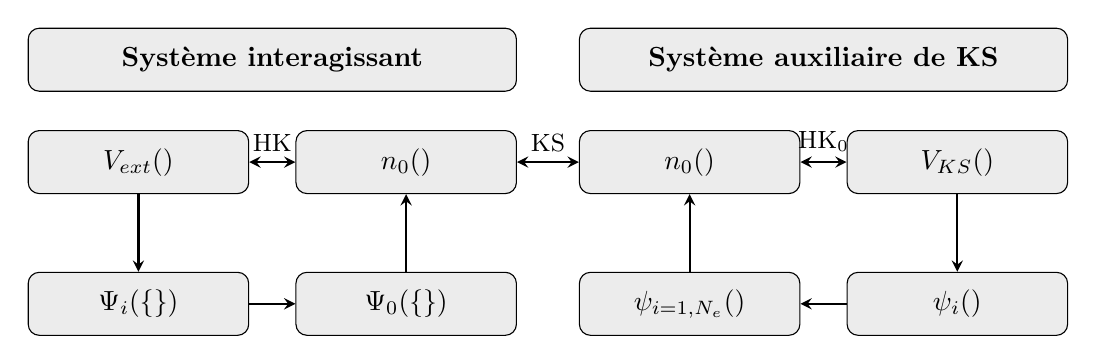
\begin{tikzpicture}[
    box/.style={rectangle, draw=black, rounded corners,
                fill=gray!15, minimum width=2.8cm,
                minimum height=0.8cm, align=center},
    arrow/.style={->, >=stealth, thick},
    darrow/.style={<->, >=stealth, thick}
]

% ---- Titres ----
\node[box, minimum width=6.2cm] at (-3.5, 2.5)
    {\textbf{Système interagissant}};
\node[box, minimum width=6.2cm] at (3.5, 2.5)
    {\textbf{Système auxiliaire de KS}};

% ---- Ligne du haut ----
\node[box] (vext)   at (-5.2,  1.2) {$V_\text{ext}(\rv)$};
\node[box] (n0l)    at (-1.8,  1.2) {$n_0(\rv)$};
\node[box] (n0r)    at ( 1.8,  1.2) {$n_0(\rv)$};
\node[box] (vks)    at ( 5.2,  1.2) {$V_\text{KS}(\rv)$};

% ---- Ligne du bas ----
\node[box] (psii)   at (-5.2, -0.6) {$\Psi_i(\{\rv\})$};
\node[box] (psi0)   at (-1.8, -0.6) {$\Psi_0(\{\rv\})$};
\node[box] (phiine) at ( 1.8, -0.6) {$\psi_{i=1,N_e}(\rv)$};
\node[box] (phii)   at ( 5.2, -0.6) {$\psi_i(\rv)$};

% ---- Flèches horizontales haut ----
\draw[darrow] (vext.east) -- (n0l.west)
    node[midway, above] {\small HK};
\draw[darrow] (n0l.east)  -- (n0r.west)
    node[midway, above] {\small KS};
\draw[darrow] (n0r.east)  -- (vks.west)
    node[midway, above] {\small HK$_0$};

% ---- Flèches verticales ----
\draw[arrow] (vext.south)   -- (psii.north);
\draw[arrow] (psi0.north)   -- (n0l.south);
\draw[arrow] (phiine.north) -- (n0r.south);
\draw[arrow] (vks.south)    -- (phii.north);

% ---- Flèches horizontales bas ----
\draw[arrow] (psii.east)  -- (psi0.west);
\draw[arrow] (phii.west)  -- (phiine.east);

\end{tikzpicture}
    \caption[Représentation schématique du système auxiliaire de Kohn-Sham.]{Représentation schématique du système auxiliaire de Kohn-Sham. La notation HK$_0$ désigne les théorèmes de HK appliqués au système auxiliaire non-interagissant. La flèche double KS donne la connexion entre les deux systèmes de sorte que chaque boîte du schéma soit reliée à toutes les autres. En conséquence, la solution du système auxiliaire donne, en théorie, toutes les propriétés du système à plusieurs corps en interaction. Figure adaptée de \cite{martinElectronicStructureBasic2004}.}
    \label{fig:ks}
\end{figure}

\newpage
\noindent\textbf{Équations de Kohn-Sham}

Le deuxième théorème de HK garantit que l'énergie de l'état fondamental du système auxiliaire de KS est le minimum de la fonctionnelle d'énergie $E_\text{KS}[n]$ définie dans l'équation \eqref{eqn:c2_EKS} et la densité qui la minimise est celle de l'état fondamental $n_0(\rv)$. En minimisant cette fonctionnelle par rapport aux fonctions d'onde sous la contrainte d'orthonormalisation $\bra{\psi_{n\kv}}\ket{\psi_{n'\kv'}}=\delta_{nn'}\delta_{\kv\kv'}$, nous arrivons aux fameuses équations de KS
\begin{equation}
    \label{eqn:c2_KS}
    \hat{H}_\text{KS}\psi_{n\kv}=\varepsilon_{n\kv}\psi_{n\kv},
\end{equation}
où $\varepsilon_{n\kv}$ est l'énergie de la fonction d'onde à un électron $\psi_{n\kv}$ et $H_\text{KS}$ est l'Hamiltonien effectif à un électron de KS
\begin{equation}
    \label{eqn:c2_HKS}
    \hat{H}_\text{KS}=-\frac{\hbar^2}{2m_e}\nabla^2+V_\text{KS}(\rv),
\end{equation}
avec le potentiel effectif de KS
\begin{align}
    \label{eqn:c2_VKS}
    V_\text{KS}(\rv)&=V_\text{ext}(\rv)+\frac{\delta E_\text{H}}{\delta n(\rv)}+\frac{\delta E_\text{XC}}{\delta n(\rv)}\notag\\
    &=V_\text{ext}(\rv)+V_\text{H}(\rv)+V_\text{XC}(\rv),
\end{align}
C'est la grande simplification de la méthode de KS: le problème à $N_e$ corps en interaction a été reformulé en $N_e$ équations indépendantes à une seule particule, dont la complexité varie linéairement avec $N_e$ plutôt qu'exponentiellement. C'est cette réduction qui rend les calculs DFT praticables.

Ces équations doivent cependant être résolues de manière auto-cohérente : le potentiel $V_\text{KS}(\rv)$ dépend de la densité $n(\rv)$ via $V_\text{H}(\rv)$ et $V_\text{XC}(\rv)$, qui est elle-même obtenue à partir des fonctions d'onde -- solutions des équations de KS. Nous détaillons cette procédure d'autocohérence (méthode SCF, de l'anglais \textit{Self-Consistent Field}) ainsi que son implémentation pratique dans la base d'ondes planes dans la section~\ref{sec:PW}.

Une fois que les équations de KS sont résolues et le problème électronique est diagonalisé, l'Hamiltonien admet une forme simple écrite dans le language de la deuxième quantification:
\begin{equation}
    \hat{H}_e = \sum_{n\kv}\varepsilon_{n\kv}\hat{c}^\dag_{n\kv}\hat{c}_{n\kv},
\end{equation}
où $\varepsilon_{n\kv}$ sont les valeurs propres de KS et $\hat{c}^\dag_{n\kv}$ et $c_{n\kv}$ sont les opérateurs de création et d'annihilation d'un électron dans la bande $n$ avec un vecteur d'onde $\kv$. Les électrons sont des fermions, ces opérateurs anticommutent entre eux. 

Nous notons enfin que les valeurs propres $\varepsilon_{n\kv}$ des équations de KS n'ont pas de signification physique directe : ce sont des multiplicateurs de Lagrange introduits pour satisfaire la condition d'orthonormalisation des fonctions d'onde, et non l'énergie nécessaire pour ajouter ou retirer des électrons du système en interaction. La seule exception est la plus haute valeur propre occupée, qui correspond à moins l'énergie d'ionisation, un résultat connu sous le nom de théorème de Janak~\cite{janakProof1978}. En pratique, ces valeurs propres sont néanmoins utilisées pour calculer les structures de bandes et les densités d'états, un usage formellement abusif dont la manifestation la plus connue est la sous-estimation systématique du gap électronique par la DFT~\cite{perdewPhysicalContentExact1983,shamDensityFunctionalTheoryEnergy1983}.

Le succès extraordinaire de la méthode de KS tient à deux facteurs : la réduction du problème à plusieurs corps en équations découplées à une particule, et le succès remarquable des approximations pour la fonctionnelle XC $E_\text{XC}[n]$ discutées à la section~\ref{sec:XC}. Les articles de HK \cite{hohenbergInhomogeneousElectronGas1964} et de KS \cite{kohnSelfConsistentEquationsIncluding1965} sont encore aujourd'hui parmi les plus cités de la \textit{Physical Review}.

\subsection{Fonctionnelles d'échange-corrélation}\label{sec:XC}

Le choix de l'approximation pour la fonctionnelle d'échange-corrélation (XC) $E_\text{XC}[n]$ a une influence significative sur les résultats des calculs DFT. Les approximations disponibles sont organisées en une hiérarchie -- l'échelle de Jacob, introduite par Perdew \cite{perdewJacobsLadderDensity2001} et illustrée à la figure \ref{fig:jacob} -- où chaque échelon incorpore davantage d'information sur la densité électronique, gagnant en précision au prix d'un coût computationnel accru. Dans cette section, nous présentons brièvement les deux premiers échelons et justifions notre choix de fonctionnelle. 
\begin{figure}[h]
    \centering
    \begin{tikzpicture}[
    rung/.style={
        draw=black,
        fill=gray!15,
        rounded corners=4pt,
        minimum width=12cm,
        minimum height=1.0cm,
        align=center,
        font=\small
    },
    arrow/.style={
        -{Stealth[length=8pt]},
        line width=1.5pt
    },
    label/.style={
        font=\small,
        align=center
    }
]

% ---- rungs (bottom to top) ----
\node[rung] (lda)  at (0,0)
    {\textbf{LDA} --- approximation de la densité locale\\
     $n(\rv)$};

\node[rung,fill=darkblue!15] (gga)  at (0,1.5)
    {\textbf{GGA} --- approximation du gradient généralisé\\
     $n(\rv)$ et $\nabla n(\rv)$};

\node[rung] (mgga) at (0,3.0)
    {\textbf{meta-GGA} --- densité d'énergie cinétique\\
     $n(\rv), \nabla n(\rv)$ et $\tau(\rv)$};

\node[rung] (hyb)  at (0,4.5)
    {\textbf{Hybrides} --- échange exact\\};

\node[rung] (rpa)  at (0,6.0)
    {\textbf{RPA / Double hybrides} --- corrélation non-locale\\
     Fonctionnelles dépendant des états inoccupés};

% ---- ground and heaven ----
\node[draw=black, fill=gray!15, rounded corners=4pt,
      minimum width=12cm, minimum height=0.7cm,
      align=center, font=\small] (earth) at (0,-1.1)
    {Théorie de Hartree};

\node[draw=black, fill=gray!15, rounded corners=4pt,
      minimum width=12cm, minimum height=0.7cm,
      align=center, font=\small] (heaven) at (0,7.1)
    {Solution exacte};

% ---- ladder poles ----
\draw[line width=2pt, black] (-5.5,-0.75) -- (-5.5,6.75);
\draw[line width=2pt, black] ( 5.5,-0.75) -- ( 5.5,6.75);

% ---- vertical arrows ----
\draw[arrow, black] (-7.0,-0.55) -- (-7.0,6.75)
    node[midway, left=4pt, label]
    {Précision\\croissante};

\draw[arrow, black] (7.0,6.75) -- (7.0,-0.55)
    node[midway, right=4pt, label]
    {Coût\\décroissant};

\end{tikzpicture}
    \caption[L'échelle de Jacob des approximations pour la fonctionnelle d'échange-corrélation.]{L'échelle de Jacob des approximations pour la fonctionnelle d'échange-corrélation. Chaque échelon de l'échelle incorpore davantage d'information sur le système électronique gagnant en précision au prix d'un coût computationnel accru. Le deuxième échelon est mis en évidence, car nous utilisons une fonctionnelle de ce niveau pour tous les calculs de ce mémoire. Figure adaptée de \cite{perdewJacobsLadderDensity2001}.}
    \label{fig:jacob}
\end{figure}


\noindent
\textbf{Premier échelon : approximation de la densité locale}

Le premier échelon de l'échelle de Jacob est l'approximation de la densité locale (LDA, de l'anglais \textit{Local Density Approximation}) proposée par Kohn et Sham eux-mêmes dans leur article fondateur de 1965 \cite{kohnSelfConsistentEquationsIncluding1965}. L'idée centrale de la LDA est d'approximer localement la fonctionnelle XC par celle d'un gaz d'électrons interagissants homogène de même densité $n$ 
\begin{equation}
    E_\text{XC}^\text{LDA}[n]=\int d^3\rv\,n(\rv)\,\varepsilon_\text{XC}^\text{hom}(n),
    \label{eqn:c1_LDA}
\end{equation}
où $\varepsilon_\text{XC}^\text{hom}(n)$ est la densité d'énergie d'échange-corrélation du gaz d'électrons homogène\footnote{Homogène signifie ici que la densité est la même partout dans le gaz : $n(\rv)=n$. La densité d'énergie d'échange-corrélation du gaz $\varepsilon_\text{XC}^\text{hom}(n)$ n'est pas une fonctionnelle, car $n$ n'est plus une fonction, d'où les parenthèses.}. Cette densité d'énergie peut être décomposée en une contribution d'échange et une contribution de corrélation : la partie d'échange est connue analytiquement \cite{martinElectronicStructureBasic2004}, tandis que la partie de corrélation a été calculée numériquement par Ceperley et Alder \cite{ceperleyGroundStateElectron1980} puis paramétrée par Perdew et Zunger \cite{perdewSelfinteractionCorrectionDensityfunctional1981}.

Malgré sa simplicité, la LDA connaît un succès remarquable pour les métaux et les semi-conducteurs. Elle souffre cependant de plusieurs limitations : elle tend à sous-estimer les constantes du réseau (\textit{overbinding}) \cite{perdewAtomsMoleculesSolids1992}, sous-estime systématiquement les gaps électroniques \cite{perdewPhysicalContentExact1983,shamDensityFunctionalTheoryEnergy1983} et ne peut décrire les interactions de van der Waals \cite{grimmeAccurateDescriptionVan2004,rapcewiczFluctuationAttractionCondensed1991} ni les systèmes à forte corrélation électronique \cite{BasisElectronTheory,imadaMetalinsulatorTransitions1998,anisimovBandTheoryMott1991,georgesDynamicalMeanfieldTheory1996}. Ces limitations ont motivé le développement du deuxième échelon.\\
\noindent
\textbf{Deuxième échelon : approximation du gradient généralisé et la PBE}

L'idée centrale de la GGA est d'aller au-delà de la LDA en incorporant non seulement la densité locale $n(\rv)$, mais aussi son gradient $\nabla n(\rv)$, afin de tenir compte de l'inhomogénéité de la densité électronique
\begin{equation}
    E_\text{XC}^\text{GGA}[n]=\int d^3\rv\,n(\rv)\,\left[\varepsilon_\text{X}^\text{hom}(n)\,F_\text{X}(n,\nabla n)+\varepsilon_\text{C}^\text{hom}(n)\,F_\text{C}(n,\nabla n)\right],
\end{equation}
où $F_\text{X}$ et $F_\text{C}$ sont les facteurs d'amplification adimensionnels pour l'échange et la corrélation respectivement qui encodent la correction due au gradient et $\varepsilon_\text{X/C}^\text{hom}(n)$ est de nouveau la densité d'énergie d'échange/corrélation d'un gaz d'électrons homogène. La fonctionnelle GGA la plus répandue est celle développée par Perdew, Burke et Ernzerhof\footnote{Matthias Ernzerhof est un professeur titulaire au département de chimie de l'Université de Montréal.} (PBE)~\cite{perdewGeneralizedGradientApproximation1996a}, dont les facteurs d'amplification sont construits à partir de conditions exactes connues sur la fonctionnelle XC, sans paramètres empiriques. Les expressions explicites de la PBE se trouvent dans l'annexe~\ref{annexe:pbe} et nous référons le lecteur à l'article original pour les dérivations. Nous utilisons cette fonctionnelle pour tous les calculs de ce mémoire.

La PBE corrige l'\textit{overbinding} systématique de la LDA et donne de très bons résultats à moindre coût computationnel~\cite{kurthMolecularSolidstateTests1999,mounetFirstprinciplesDeterminationStructural2005a}, ce qui en fait une fonctionnelle de choix pour ce mémoire. Pour le graphène, la PBE décrit correctement les propriétés électroniques et vibrationnelles. En particulier, la PBE reproduit fidèlement le gap nul du graphène : les cônes de Dirac au point $\Kv$ de la zone Brillouin\footnote{Non pas parce que la PBE reproduit exactement les effets d'échange-corrélation, mais parce que les cônes de Dirac sont protégés par la symétrie du réseau hexagonal. En effet, même un simple modèle \textit{tight-binding}, qui néglige complètement les interactions électron-électron, reproduit les cônes de Dirac. C'est une propriété d'origine purement géométrique.}. Les interactions de van der Waals, toujours absentes dans la PBE, sont négligeables pour le graphène monocouche étudié ici. De plus, les électrons $\pi$ des orbitales $p_z$ du carbone, qui dominent largement les propriétés électroniques du graphène, sont délocalisés et faiblement corrélés, ce qui rend la PBE tout à fait appropriée.  Les fonctionnelles des échelons supérieurs apportent des corrections négligeables aux systèmes de graphènes étudiés dans ce mémoire, à un coût computationnel prohibitif pour les super-cellules nécessaires à la modélisation des défauts, ce qui renforce notre choix de la PBE. L'article PBE \cite{perdewGeneralizedGradientApproximation1996a} est encore aujourd'hui l'un des plus cités de la \textit{Physical Review}.

Notons finalement que la sous-estimation du gap électronique demeure une limitation fondamentale de toutes les fonctionnelles locales ou semi-locales, incluant la PBE. Pour une description quantitative des intensités Raman résonantes, il sera probablement nécessaire de corriger les valeurs propres de Kohn-Sham à l'aide de l'approximation $GW$ \cite{hedinNewMethodCalculating1965,hybertsenElectronCorrelationSemiconductors1986}, qui traite les effets d'échange et de corrélation via la fonction de Green $G$ et l'interaction de Coulomb écrantée $W$, et qui donne des gaps qui sont en excellent accord avec l'expérience.

\subsection{Pseudo-potentiels}\label{sec:PP}

Le potentiel externe $V_\text{ext}(\rv)$, qui décrit l'interaction de Coulomb entre les électrons et les noyaux, diverge en $1/r$ au voisinage des ions. Cette singularité génère des états de c\oe ur fortement oscillants près des noyaux, auxquels les fonctions d'onde des électrons de valence héritent d'oscillations rapides afin de satisfaire à la condition d'orthonormalité. Ces électrons de c\oe ur, fortement liés aux noyaux et chimiquement inertes, contribuent peu aux propriétés d'intérêt et augmentent considérablement le coût des calculs. L'approximation des pseudo-potentiels~\cite{phillipsEnergyBandInterpolationScheme1958,phillipsNewMethodCalculating1959} résout ces deux problèmes simultanément : les électrons de c\oe ur sont absorbés dans les noyaux pour former les ions et leur effet sur les électrons de valence est encodé dans un pseudo-potentiel $V_\text{PP}(\rv)$ qui remplace le potentiel de Coulomb divergent par un potentiel plus lisse, réduisant à la fois le nombre d'électrons à traiter explicitement et la complexité des fonctions d'onde de valence.

On distingue principalement trois grandes catégories de pseudo-potentiels : les pseudo-potentiels à conservation de norme (NC, de l'anglais \textit{Norm-Conserving}) \cite{hamannNormConservingPseudopotentials1979}, les pseudo-potentiels \textit{ultrasoft} de Vanderbilt \cite{vanderbiltSoftSelfconsistentPseudopotentials1990} et la méthode des ondes augmentées projetées (PAW, de l'anglais \textit{Projector Augmented Waves}) de Blöchl \cite{blochlProjectorAugmentedwaveMethod1994}. Pour tous les calculs effectués dans ce mémoire nous utilisons des pseudo-potentiels de NC de la famille ONCV (de l'anglais \textit{Optimized Norm-Conserving Vanderbilt}) tirés de la bibliothèque PseudoDojo \cite{vansettenPseudoDojoTrainingGrading2018}, qui offrent un excellent compromis entre précision et efficacité computationnelle. Les pseudo-potentiels NC satisfont la condition de conservation de la norme
\begin{equation}
    \int_0^{r_c}dr\,|\psi_\ell^\text{PP}(r)|^2r^2=\int_0^{r_c}dr\,|\psi_\ell^\text{AE}(r)|^2r^2,
    \label{eqn:c2_nc}
\end{equation}
où $\psi_\ell^\text{AE}(r)$ est la fonction d'onde de valence que nous obtiendrions si nous résolvions les équations de KS avec le vrai potentiel de Coulomb et en traitant tous les électrons explicitement (l'indice AE vient de l'anglais \textit{All Electrons}), $\psi_\ell^\text{PP}(r)$ est la fonction d'onde obtenue en résolvant le problème dans l'approximation des pseudo-potentiels et $r_c$ est un rayon de coupure au-delà duquel les deux fonctions d'onde coïncident exactement. Cette condition garantit la bonne reproduction de la densité de charge dans la région de c\oe ur ainsi qu'une bonne transférabilité du pseudo-potentiel à différents environnements chimiques~\cite{hamannGeneralizedNormconservingPseudopotentials1989,troullierEfficientPseudopotentialsPlanewave1991}.

\noindent\textbf{Pseudo-potentiels ONCV et forme de Kleinman-Bylander}

Dans les codes DFT modernes, la forme séparable proposée par Kleinman et Bylander (KB)~\cite{kleinmanEfficaciousFormModel1982} pour les pseudo-potentiels NC est généralement employée, car elle réduit radicalement le nombre d'opérations nécessaires pour l'application de la partie non-locale de l'Hamiltonien, ainsi que la mémoire nécessaire pour stocker l'opérateur. Dans l'approximation des pseudo-potentiels, l'interaction des électrons de valence avec les ions est remplacée par un pseudo-potentiel total
\begin{equation}
    V_\text{PP}(\rv)=\sum_\alpha V_\text{PP}^{(\alpha)}(\rv-\bm{\tau}_\alpha),
    \label{eqn:c2_pp_approx}
\end{equation}
où la somme court sur tous les ions $\alpha$ de la cellule unitaire et $\bm{\tau}_\alpha$ dénote leur position. Dans la forme de KB, chaque contribution ionique se décompose en une partie locale et une partie non-locale
\begin{equation}
    V^{(\alpha)}_\text{PP}(\rv) = V^{(\alpha)}_\text{PPL}(\rv)+\underbrace{\sum_{i\ell m}\ket{\beta_{i\ell m}^{(\alpha)}}E_{i\ell}^{(\alpha)}\bra{\beta_{i\ell m}^{(\alpha)}}}_{=\hat{V}_\text{PPNL}^{(\alpha)}}.
    \label{eqn:c1_VKB}
\end{equation}
La partie locale $V_\text{PPL}(\rv)$ est un potentiel central à symétrie sphérique qui reproduit le potentiel de Coulomb $-Z_\text{val}/r$ loin de la région de c\oe ur et est plus lisse à l'intérieur. Dans la partie non-locale, $\ell$ est le nombre quantique de moment cinétique orbital, $m=-\ell,\dots,\ell$ est le nombre quantique magnétique et $i$ indexe les multiples projecteurs par canal $\ell$. C'est précisément ce qui distingue les ONCV des NC classiques, qui ne possèdent qu'un seul projecteur par canal. Les énergies de KB $E_{i\ell}^{(\alpha)}$ mesurent la force de la partie non-locale par rapport à la partie locale et les projecteurs de KB $\beta_{i\ell m}^{(\alpha)}(\rv)=\bra{\rv}\ket{\beta_{i\ell m}^{(\alpha)}}$ sont des fonctions à courte portée centrées sur l'ion $\alpha$, dont la structure est
\begin{equation}
    \beta_{i\ell m}^{(\alpha)}(\rv)=\frac{1}{|\rv-\bm{\tau}_\alpha|}\beta_{i\ell}^{(\alpha)}(|\rv-\bm{\tau}_\alpha|)Y_{\ell}^m(\theta,\phi),
    \label{eqn:c2_betar}
\end{equation}
où $Y_\ell^m(\theta, \phi)$ sont les harmoniques sphériques et $\theta$ et $\phi$ sont les angles en coordonnées sphériques du vecteur $\rv-\bm{\tau}_\alpha$. La partie locale et les projecteurs radiaux du pseudo-potentiel ONCV pour un atome de carbone sont illustrés à la figure~\ref{fig:KB}.

\begin{figure}[t]
    \centering
    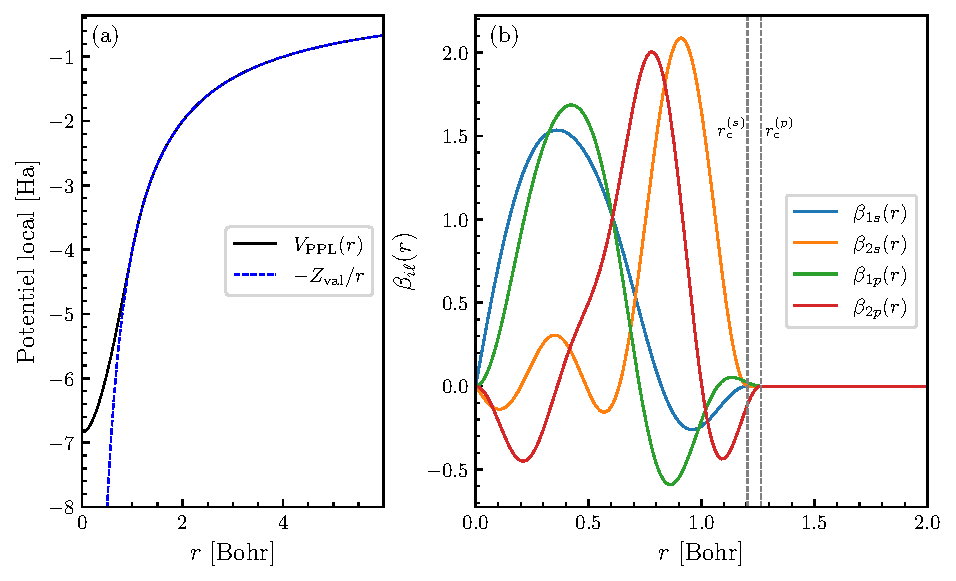
\includegraphics{figures/KB_projectors_C.pdf}
    \caption[Illustration de la partie locale et non-locale du pseudo-potentiel pour un atome
    de carbone.]{Illustration de la partie locale et non-locale du pseudo-potentiel pour un atome de carbone. (a) Comparaison entre la partie locale du pseudo-potentiel $V_\text{PPL}(r)$ et le potentiel de Coulomb $-Z_\text{val}/r$ où $Z_\text{val}=4$ est la charge des électrons de valence du carbone. Notons que $V_\text{PPL}(r)$ corrige la divergence du potentiel de Coulomb à l'origine. (b) Partie radiale des projecteurs de KB $\beta_{i\ell}(r)$, qui s'annulent au-delà des rayons de coupure $r_c^{(s)}$ et $r_c^{(p)}$. Le
    pseudo-potentiel est de type ONCV \textit{stringent} pour la fonctionnelle XC PBE, tiré de la bibliothèque PseudoDojo 
    \cite{vansettenPseudoDojoTrainingGrading2018}.}
    \label{fig:KB}
\end{figure}

La décomposition du pseudo-potentiel en une partie locale et une partie non-locale se répercute directement sur le potentiel de KS, qui lui aussi se sépare en deux parties : 
\begin{equation}
    V_\text{KS}(\rv)=V_\text{L}(\rv)+V_\text{NL},
    \label{eqn:c2_VKS_lnl}
\end{equation}
où la partie locale du potentiel regroupe les contributions d'Hartree, d'échange-corrélation et la partie locale du pseudo-potentiel
\begin{equation}
    V_\text{L}(\rv) = V_\text{H}(\rv)+V_\text{XC}(\rv)+\sum_\alpha V_\text{PPL}^{(\alpha)}(\rv-\bm{\tau}_\alpha),
    \label{eqn:c2_VL}
\end{equation}
et la partie non-locale est entièrement due aux projecteurs de KB
\begin{equation}
    \hat{V}_\text{NL}=\sum_\alpha\sum_{i\ell m}\ket{\beta_{i\ell m}^{(\alpha)}}E_{i\ell}^{(\alpha)}\bra{\beta_{i\ell m}^{(\alpha)}}.
\end{equation}
Nous aurons besoin de ces expressions lors du calcul des éléments de matrice de couplage électron-défaut au chapitre \ref{chap:défauts}, ainsi que pour la solution des équations de KS, présentée dans la prochaine section.

\subsection{Base d'ondes planes et résolution des équations de Kohn-Sham dans l'espace réciproque}\label{sec:PW}

Dans cette section, nous voyons comment résoudre les équations de Kohn-Sham en pratique dans l'espace réciproque. À cet effet, il est nécessaire de faire l'expansion de la fonction d'onde dans une base complète. Pour les solides cristallins, une base naturelle est celle des ondes planes, puisqu'elle exploite la symétrie de translation discrète des cristaux.

\noindent\textbf{Base d'ondes planes}

D'après le théorème de Bloch (cf. section~\ref{sec:2.1.2}), les fonctions d'onde de KS prennent la forme
\begin{equation}
    \psi_{n\kv}(\rv)=e^{i\kv\cdot\rv}u_{n\kv}(\rv),
    \label{eqn:c2_bloch_pt2}
\end{equation}
où la fonction périodique de Bloch possède la même périodicité que le solide : $u_{n\kv}(\rv+\Rv_\ell) = u_{n\kv}(\rv)$. Grâce à cette invariance sous translation discrète par un vecteur du réseau cristallin, il est possible de faire son expansion en série de Fourier avec les vecteurs $\Gv$ du réseau réciproque seulement
\begin{equation}
    u_{n\kv}(\rv)=\frac{1}{\sqrt{\Omega_\text{BvK}}}\sum_{\Gv}C_{n\kv}(\Gv)e^{i\Gv\cdot\rv},
    \label{eqn:c2_uPW}
\end{equation}
où $\Omega_\text{BvK}$ est le volume du cristal et $C_{n\kv}(\Gv)$ sont les coefficients de l'expansion en série de Fourier, de sorte que la fonction d'onde de KS s'écrit comme une combinaison linéaire d'ondes planes
\begin{equation}
    \psi_{n\kv}(\rv)=\frac{1}{\sqrt{\Omega_\text{BvK}}}\sum_{\Gv}C_{n\kv}(\Gv)e^{i(\kv+\Gv)\cdot\rv}.
    \label{eqn:c2_psiPW}
\end{equation}
La base d'onde plane est un choix naturel pour les solides périodiques~\cite{carUnifiedApproachMolecular1985,martinElectronicStructureBasic2004} : elle est complète, orthonormée, et compatible avec les transformées de Fourier rapides (FFT, de l'anglais \textit{Fast Fourier Transform}) qui permettent de passer efficacement entre l'espace réel et l'espace réciproque. Le problème se réduit donc à la détermination des coefficients $C_{n\kv}(\Gv)$.

Formellement, il faut un nombre infini d'ondes planes pour représenter la fonction d'onde. En pratique, nous tronquons la série en introduisant une énergie de coupure $E_\text{cut}$ telle que seules les ondes planes satisfaisant
\begin{equation}
    \frac{\hbar^2}{2m_e}|\kv+\Gv|^2\leq E_\text{cut}.
    \label{eqn:c2_Ecut}
\end{equation}
sont retenues. Une valeur de $E_\text{cut}$ plus élevée améliore la précision des calculs au prix d'un coût numérique plus grand. Notons qu'un très grand nombre d'ondes planes seraient nécessaires pour représenter les oscillations rapides des fonctions d'onde près des noyaux. Heureusement, ce problème est résolu par l'approximation des pseudo-potentiels (cf. section~\ref{sec:PP}), qui garantit des fonctions d'onde lisses dans la région de c\oe ur.

Finalement, nous souhaitons que les fonctions d'onde soient orthonormales sur l'ensemble du système, soit le volume du cristal $\Omega_\text{BvK}$ 
\begin{equation}
    \int_{\Omega_\text{BvK}}d^3\rv\,\psi_{n\kv}^*(\rv)\psi_{n'\kv'}(\rv)=\delta_{nn'}\delta_{\kv\kv'}.
    \label{eqn:c2_psi_norm}
\end{equation}
En remplaçant les fonctions d'onde par leur expansion en ondes planes \eqref{eqn:c2_psiPW}, nous pouvons montrer que les coefficients d'expansion satisfont la relation
\begin{equation}
    \sum_\Gv C_{n\kv}^*(\Gv)C_{n'\kv}(\Gv)=\delta_{nn'}.
    \label{eqn:c2_C_norm}
\end{equation}
Nous avons maintenant tous les ingrédients nécessaires pour écrire les équations de KS dans la base d'ondes planes et les résoudre formellement.

\noindent\textbf{Équations de Kohn-Sham dans la base d'ondes planes}

Nous souhaitons écrire les équations de KS (équations \eqref{eqn:c2_KS}--\eqref{eqn:c2_VKS}) dans la base d'ondes planes. Premièrement, en substituant la forme de Bloch pour la fonction d'onde, nous obtenons les équations de KS en termes de $u_{n\kv}(\rv)$,
\begin{equation}
    \left(-\frac{\hbar^2}{2m_e}(\nabla+i\kv)^2+V_\text{KS}(\rv)\right)u_{n\kv}(\rv)=\varepsilon_{n\kv}u_{n\kv}(\rv),
    \label{eqn:c2_UKS}
\end{equation}
Ensuite, en utilisant l'expansion de $u_{n\kv}(\rv)$ en ondes planes (équation \eqref{eqn:c2_uPW}) dans l'équation précédente et en utilisant l'expansion de $V_\text{KS}(\rv)$ en série de Fourier 
\begin{equation}
    V_\text{KS}(\rv)=\sum_{\Gv}\tilde{V}_\text{KS}(\Gv)e^{i\Gv\cdot\rv},
    \label{eqn:c2_VKSG}
\end{equation}
nous obtenons les équations de KS dans la base d'ondes planes
\begin{equation}
    \sum_{\Gv'}\left(\frac{\hbar^2}{2m_e}|\kv+\Gv|^2\delta_{\Gv\Gv'}+\tilde{V}_\text{KS}(\Gv-\Gv')\right)C_{n\kv}(\Gv')=\varepsilon_{n\kv}C_{n\kv}(\Gv).
    \label{eqn:c2_KSPW}
\end{equation}
Notons que l'expansion en série de Fourier du potentiel de KS ne se fait qu'avec les vecteurs du réseau réciproque $\Gv$, car $V_\text{KS}$ est aussi invariant sous une translation par un vecteur du réseau cristallin $\Rv_\ell$. L'équation de KS dans la base d'ondes planes, l'équation \eqref{eqn:c2_KSPW}, est formellement un problème aux valeurs propres matriciel $H^{(\kv)}_{\Gv\Gv'}\mathbf{C}=\varepsilon\mathbf{C}$, où la matrice Hamiltonienne est donnée par
\begin{equation}
    H^{(\kv)}_{\Gv\Gv'}=\frac{\hbar^2}{2m_e}|\kv+\Gv|^2\delta_{\Gv\Gv'}+\tilde{V}_\text{KS}(\Gv-\Gv').
    \label{eqn:c2_HGG}
\end{equation}
Cette matrice Hamiltonienne est de taille $N_\text{PW}\times N_\text{PW}$, où $N_\text{PW}$ est le nombre d'ondes planes déterminé par la coupure d'énergie cinétique $E_\text{cut}$ de l'équation \eqref{eqn:c2_Ecut} et dépend généralement du point $\kv$ considéré. Le paramètre $E_\text{cut}$ contrôle donc la taille du problème aux valeurs propres à résoudre à chaque itération du cycle SCF. En pratique, $N_\text{PW}$ peut atteindre plusieurs milliers à plusieurs dizaines de milliers d'ondes planes selon le système et la précision souhaitée. Notons également que la matrice Hamiltonienne dépend de $\kv$ et doit être construite pour chaque $\kv$ de la première IBZ. Le potentiel $\tilde{V}_\text{KS}(\Gv-\Gv')$ est mis à jour à chaque itération du cycle SCF à partir de la nouvelle densité $n_\text{out}(\rv)$ que nous décrivons en détail dans ce qui suit et est illustré à la figure \ref{fig:scf_PW}. Le cycle SCF dans la base d'ondes planes se déroule comme suit:
\begin{enumerate}
    \item Commencer avec une estimation de la densité initiale $n_\text{in}(\rv)$.
    \item Transformer la densité d'entrée dans l'espace réciproque à l'aide d'une FFT:
    \begin{equation*}
        n_\text{in}(\rv) \xrightarrow{\text{FFT}} \tilde{n}_\text{in}(\Gv).
    \end{equation*}
    \item Calculer les composantes de Fourier de la partie locale du potentiel de KS. La partie de Hartree est obtenue directement dans l'espace réciproque via l'équation de Poisson
    \begin{equation*}
        \tilde{V}_\text{H}(\Gv)=\frac{4\pi e^2}{|\Gv|^2}\tilde{n}_\text{in}(\Gv),
    \end{equation*}
    la partie d'échange-corrélation $\tilde{V}_\text{XC}(\Gv)$ est obtenue par la FFT de $V_\text{XC}[n_\text{in}(\rv)]$ calculé dans l'espace réel, et la partie locale du pseudo-potentiel $\tilde{V}_\text{PPL}(\Gv)$ est précalculée en faisant la FFT de $V_\text{PPL}(\rv)$, qui ne dépend pas de la densité. La partie locale est assemblée dans l'espace réciproque par la somme de ces trois termes
    \begin{equation*}
        \tilde{V}_\text{L}(\Gv) = \tilde{V}_\text{H}(\Gv)+\tilde{V}_\text{XC}(\Gv)+\tilde{V}_\text{PPL}(\Gv).
    \end{equation*}
    \item Précalculer la partie non-locale du potentiel de KS pour chaque $\kv$, car elle ne dépend pas de la densité
    \begin{equation*}
        \tilde{V}_\text{NL}^{(\kv)}(\Gv, \Gv')=\sum_\alpha\sum_{i\ell m}\tilde{\beta}_{i\ell m}^{(\alpha)}(\kv+\Gv)E_{i\ell}^{(\alpha)}\tilde{\beta}^{*(\alpha)}_{i\ell m}(\kv+\Gv').
    \end{equation*}
    La dérivation de cette expression est présentée dans le chapitre \ref{chap:défauts} dans le contexte du calcul des éléments de matrice électron-défaut.
    \item Construire la matrice Hamiltonienne pour chaque point $\kv$ de la première BZ
    \begin{equation*}
        H^{(\kv)}_{\Gv\Gv'}=\frac{\hbar^2}{2m_e}|\kv+\Gv|^2\delta_{\Gv\Gv'}+\tilde{V}_\text{L}(\Gv-\Gv')+\tilde{V}^{(\kv)}_\text{NL}(\Gv,\Gv'),
    \end{equation*}
    et diagonaliser pour obtenir les coefficients $C_{n\kv}(\Gv)$ et les valeurs propres $\varepsilon_{n\kv}$. La diagonalisation se fait itérativement à l'aide d'algorithmes de sous-espace.
    \item Calculer les fonctions d'ondes dans l'espace réel à partir des coefficients des ondes planes à l'aide d'une FFT inverse
    \begin{equation*}
        C_{n\kv}(\Gv)\xrightarrow{\text{FFT}^{-1}}\psi_{n\kv}(\rv).
    \end{equation*}
    \item Calculer la nouvelle densité électronique à partir des fonctions d'onde dans l'espace réel
    \begin{equation*}
        n_\text{out}(\rv)=\sum_{n\kv}f_{n\kv}|\psi_{n\kv}(\rv)|^2,
    \end{equation*}
    \item Construire la nouvelle densité d'entrée à partir de $n_\text{in}$ et $n_\text{out}$ via un schéma de \textit{mixing}.
    \item Si la différence entre $n_\text{in}$ et $n_\text{out}$ est inférieure à une tolérance spécifiée, ou d'autres critères de convergence sont satisfaits, passer à l'étape 10. Autrement, retourner à l'étape 2. 
    \item Calculer les propriétés de l'état fondamental.
\end{enumerate}
\begin{figure}[t]
    \centering
    \hspace{2.5cm}
    \begin{tikzpicture}[
    box/.style={rectangle, draw=black, rounded corners,
                fill=gray!15, minimum width=6.5cm,
                minimum height=1.3cm, align=center, font=\small, inner sep=6pt},
    sidebox/.style={rectangle, draw=black, rounded corners,
                fill=gray!15, minimum width=3.8cm,
                minimum height=0.85cm, align=center, font=\small},
    decision/.style={diamond, draw=black, fill=darkblue!15,
                     aspect=3, align=center, font=\small},
    arrow/.style={->, >=stealth, thick},
    label/.style={font=\small, midway},
]

\def\sep{1.55}

% ---- Nœuds principaux ----
\node[box] (nin)    at (0,  0)           {$n_\text{in}^{(i)}(\rv)$};
\node[font=\scriptsize\bfseries, anchor=north west] 
    at (nin.north west) {(1)};

\node[box] (ninG)   at (0, -1*\sep)      {$\tilde{n}_\text{in}(\Gv)$};
\node[font=\scriptsize\bfseries, anchor=north west] 
    at (ninG.north west) {(2)};

\node[box] (VL)     at (0, -2*\sep)      {$\tilde{V}_\text{L}(\Gv)
                                           =\tilde{V}_\text{H}(\Gv)
                                           +\tilde{V}_\text{XC}(\Gv)
                                           +\tilde{V}_\text{PPL}(\Gv)$};
\node[font=\scriptsize\bfseries, anchor=north west] 
    at (VL.north west) {(3)};

\node[box] (H)      at (0, -3.3*\sep)    {$H^{(\kv)}_{\Gv\Gv'}
                                           \;\longrightarrow\;
                                           C_{n\kv}(\Gv),\;
                                           \varepsilon_{n\kv}$};
\node[font=\scriptsize\bfseries, anchor=north west] 
    at (H.north west) {(5)};

\node[box] (psi)    at (0, -4.6*\sep)    {$\psi_{n\kv}(\rv)$};
\node[font=\scriptsize\bfseries, anchor=north west] 
    at (psi.north west) {(6)};

\node[box] (nout)   at (0, -5.6*\sep)    {$n_\text{out}(\rv)
                                           =\sum_{n\kv}f_{n\kv}
                                           |\psi_{n\kv}(\rv)|^2$};
\node[font=\scriptsize\bfseries, anchor=north west] 
    at (nout.north west) {(7)};

\node[box] (mix)    at (0, -6.6*\sep)    {Mixing $\;\longrightarrow\;
                                           n_\text{in}^{(i+1)}(\rv)$};
\node[font=\scriptsize\bfseries, anchor=north west] 
    at (mix.north west) {(8)};

\node[decision](conv) at (0, -7.8*\sep)  {Convergé?};
\node[box] (props)  at (0, -9.2*\sep)    {Propriétés de l'état fondamental};
\node[font=\scriptsize\bfseries, anchor=north west] 
    at (props.north west) {(10)};

% ---- Nœuds latéraux (précalculés) ----
\node[sidebox] (VPPL) at (6.2, -2*\sep)
    {$\tilde{V}_\text{PPL}(\Gv)$\\(précalculé)};
\node[font=\scriptsize\bfseries, anchor=north west] 
    at (VPPL.north west) {(3)};
\node[sidebox] (VNL)  at (6.2, -3.3*\sep)
    {$\tilde{V}_\text{NL}^{(\kv)}(\Gv,\Gv')$\\(précalculé)};
\node[font=\scriptsize\bfseries, anchor=north west] 
    at (VNL.north west) {(4)};

% ---- Flèches flux principal ----
\draw[arrow] (nin)   -- (ninG)
    node[label, right] {FFT};
\draw[arrow] (ninG)  -- (VL);
\draw[arrow] (VL)    -- (H);
\draw[arrow] (VPPL)  -- (VL);
\draw[arrow] (VNL)   -- (H);
\draw[arrow] (H)     -- (psi)
    node[label, right] {FFT$^{-1}$};
\draw[arrow] (psi)   -- (nout);
\draw[arrow] (nout)  -- (mix);
\draw[arrow] (mix)   -- (conv);
\draw[arrow] (conv)  -- (props)
    node[label, right] {Oui};

% ---- Flèche de retour (boucle SCF) ----
\draw[arrow] (conv.west)
    -- ++(-2.5, 0)
    |- (nin.west)
    node[pos=0.01, right, font=\small] {Non};

% ---- Rectangle délimitant la boucle SCF ----
\draw[dashed, gray, rounded corners]
    (-4.0, 1.15) rectangle (4.0, -7.15*\sep);
\node[font=\small\itshape, gray] at (-2.8, 0.85) {Boucle SCF};

\end{tikzpicture}
    \caption[Représentation schématique du cycle SCF pour la résolution des équations de KS dans la base d'ondes planes.]{Représentation schématique du cycle SCF pour la résolution des équations de KS dans la base d'ondes planes.}
    \label{fig:scf_PW}
\end{figure}
Nous détaillons maintenant les ingrédients clés de ce cycle: les algorithmes de diagonalisation (étape 5), le facteur d'occupation (étape 7), le schéma de \textit{mixing} (étape 8) et l'échantillonnage de la BZ, c'est-à-dire comment choisir les points $\kv$ pour construire la matrice Hamiltonienne.

\noindent\textbf{Algorithmes de diagonalisation itératifs}

À l'étape 5 de chaque itération du cycle SCF, il faut diagonaliser la matrice Hamiltonnienne $H^{(\kv)}(\Gv,\Gv')$ de taille $N_\text{PW}\times N_\text{PW}$ pour chaque point $\kv$ de la BZ. Une diagonalisation exacte par des méthodes directes a un coût variant en $N_\text{PW}^3$ ce qui est prohibitif pour des systèmes où il faut plusieurs dizaines de milliers d'ondes planes. Heureusement, seules les $N_\text{bandes}\ll N_\text{PW}$ valeurs propres les plus basses sont nécessaires pour construire la densité électronique, car seuls les états occupés contribuent à la densité. Une première famille de méthodes itératives est celle du gradient conjugué~\cite{hestenesMethodsConjugateGradients}, qui minimise l'énergie de chaque état $\psi_{n\kv}$ individuellement dans l'espace des ondes planes par descente de gradient préconditionné. Une deuxième famille, plus performante en pratique, est celle des méthodes de sous-espace itératives : l'algorithme de Davidson~\cite{davidsonIterativeCalculationFew1975} part d'un sous-espace de petite dimension et l'enrichit itérativement en ajoutant des vecteurs de correction jusqu'à la convergence des valeurs propres cibles. L'algorithme LOBPCG~\cite{OptimalPreconditionedEigensolver} (de l'anglais \textit{Locally Optimal Block Preconditioned Conjugate Gradient}) opère sur une bloc de vecteurs simultanément et est particulièrement efficace sur des architectures parallèles. Ces méthodes ramènent le coût computationnel à $\mathcal{O}(N_\text{PW} N_\text{bandes}^2)$, une réduction considérable de la complexité. 

\newpage
\noindent\textbf{Facteur d'occupation et \textit{smearing}}

Le calcul de la densité électronique à l'étape 7 de chaque itération du cycle SCF requiert une somme de tous les états occupés de la BZ. Pour un isolant et un semi-conducteur, dont le gap électronique différencie clairement les états occupés des états inoccupés, le facteur d'occupation est simplement une fonction de Heaviside
\begin{equation}
    f_ {n\kv}=\Theta(\varepsilon_F-\varepsilon_{n\kv}),
    \label{eqn:c2_smearing_heaviside}
\end{equation}
où $\varepsilon_F$ est l'énergie de Fermi (l'énergie de l'état le plus haut en énergie occupé). Pour les métaux et les semi-métaux qui ne possèdent pas de gap, l'histoire se complique. Le niveau de Fermi traverse des bandes et la fonction Heaviside est discontinue à la surface de Fermi : un petit changement de $\varepsilon_F$ entre deux itérations du cycle SCF peut faire basculer des états d'occupés à non-occupés, introduisant des discontinuités dans la densité et déstabilisant le cycle. Pour remédier à ce problème, nous remplaçons la fonction de Heaviside par une fonction d'occupation lissée $f_{n\kv}(\sigma)$ paramétrée par un facteur d'élargissement $\sigma$, qui joue un peu le rôle de la température pour l'occupation des états électroniques. Cette température n'est pas physique et introduit des erreurs dans les calculs, en échange d'une convergence plus rapide. Il existe plusieurs formes de $f_{n\kv}$. La plus naturelle est la distribution de Fermi-Dirac
\begin{equation}
    f_{n\kv}^\text{FD}(\sigma)=\frac{1}{e^{(\varepsilon_{n\kv}-\varepsilon_F)/\sigma}+1},
    \label{eqn:c2_smearing_FD}
\end{equation}
puisque les électrons sont des particules fermioniques et obéissent à la statistique de Fermi-Dirac à température finie, avec $\sigma=k_B T$ jouant le rôle de la température. La distribution de Fermi-Dirac fait une erreur de l'ordre de $e^{-1/\sigma}$. Un autre choix est le \textit{smearing} Gaussien
\begin{equation}
    f_{n\kv}^\text{G}(\sigma)=\frac{1}{2}\left[1-\erf\left(\frac{\varepsilon_{n\kv}-\varepsilon_F}{\sigma}\right)\right],
    \label{eqn:c2_smearing_gaussien}
\end{equation}
où erf est la fonction d'erreur, soit la primitive de la Gaussienne. Le \textit{smearing} Gaussien fait une erreur de l'ordre de $\sigma^2$. Methfessel et Paxton (MP)~\cite{methfesselHighprecisionSamplingBrillouinzone1989} ont systématiquement amélioré le \textit{smearing} Gaussien en ajoutant des corrections polynomiales
\begin{equation}
    f_{n\kv}^\text{MP}(\sigma)=\frac{1}{2}\left[1-\erf\left(\frac{\varepsilon_{n\kv}-\varepsilon_F}{\sigma}\right)\right]+\sum_{n=1}^NA_nH_{2n-1}\left(\frac{\varepsilon_{n\kv}-\varepsilon_F}{\sigma}\right)e^{-(\varepsilon_{n\kv}-\varepsilon_F)^2/\sigma^2},
    \label{eqn:c2_smearing_MP}
\end{equation}
où $H_n$ sont les polynômes d'Hermite et $A_n$ sont des coefficients choisis de sorte que l'erreur est de l'ordre de $\sigma^{2N+2}$. Dans la très grande majorité des cas, $N=1$ est utilisé. Notons que le \textit{smearing} MP n'est pas une vraie fonction d'occupation : elle peut prendre des valeurs négatives ou supérieures à 1 pour des grands $\sigma$. Finalement, le \textit{smearing} de Marzari-Vanderbilt (MV)~\cite{marzariThermalContractionDisordering1999}, aussi appelé \textit{cold smearing},
\begin{equation}
    f_{n\kv}^{\text{MV}}(\sigma)=\frac{1}{2}\left[1-\erf\left(\frac{\varepsilon_{n\kv}-\varepsilon_F}{\sigma}\right)\right]+\frac{1}{\sqrt{2\pi}}\left(\frac{\varepsilon_{n\kv}-\varepsilon_F}{\sigma}\right)e^{-((\varepsilon_{n\kv}-\varepsilon_F)/\sigma+1/\sqrt{2})^2},
    \label{eqn:c2_smearing_MV}
\end{equation}
fait une erreur de l'ordre de $\sigma^2$. Cependant, le décalage de $1/\sqrt{2}$ est choisi de sorte que le facteur d'occupation MV reste dans l'intervalle $[0,1]$ ce qui est physiquement sensé et minimise l'erreur sur l'énergie libre. \textit{A priori}, il n'y pas de prescription pour choisir le schéma de \textit{smearing} pour un système donné. Il faut tester chaque schéma individuellement afin d'identifier celui 
qui converge le plus rapidement vers la limite $\sigma\to 0$, ce que 
nous faisons à la section~\ref{sec:electron_results}.

\noindent\textbf{Schéma de \textit{mixing}}

À l'étape 8 de chaque itération du cycle SCF, la densité de sortie $n_\text{out}(\rv)$ est généralement différente de la densité d'entrée $n_\text{in}(\rv)$. Utiliser directement la densité de sortie comme nouvelle densité d'entrée mène typiquement à des oscillations ou à la divergence du cycle. Pour assurer la convergence, il est nécessaire de construire la nouvelle densité en combinant $n_\text{in}$ et $n_\text{out}$ via un schéma de \textit{mixing}. Le plus simple est le \textit{mixing} linéaire
\begin{equation}
    n_\text{in}^{(i+1)}(\rv)=(1-\beta)n_\text{in}^{(i)}(\rv)+\beta n_\text{out}^{(i)}(\rv),
    \label{eqn:c2_mixing_lineaire}
\end{equation}
où $\beta\in[0,1]$ est le paramètre de \textit{mixing}. Un petit $\beta$ stabilise le cycle, mais ralentit la convergence, tandis qu'un $\beta$ plus grand accélère la convergence, mais risque de déstabiliser le cycle. Le choix de $\beta$ par essai-erreur est généralement suffisant puisque la même valeur de $\beta$ s'applique pour plusieurs systèmes similaires. Des schémas plus sophistiqués exploitent l'historique des itérations précédentes pour accélérer la convergence : le \textit{mixing} de Pulay~\cite{pulayConvergenceAccelerationIterative1980} (aussi connu sous le nom de DIIS, de l'anglais \textit{Direct Inversion in the Iterative Subspace}) minimise le résidu $R^{(i)}=n_\text{out}^{(i)}-n_\text{in}^{(i)}$ dans le sous-espace engendré par les itérations
précédentes, tandis que la méthode de Broyden~\cite{Broyden1965Class} construit une approximation du Jacobien inverse du résidu. 

Pour les systèmes métalliques et semi-métalliques comme le graphène, le cycle SCF est sujet au problème de \textit{charge sloshing} : une instabilité où la densité électronique oscille entre les itérations plutôt que de converger, particulièrement prononcé pour les états proches du niveau de Fermi. Un paramètre $\beta$ plus petit atténue ce problème au prix d'une convergence plus lente, tandis que les schémas de Pulay et Broyden sont un peu plus efficaces que le \textit{mixing} linéaire en préconditionnant implicitement le résidu via l'historique des itérations. Pour ces raisons, nous utilisons le schéma de Broyden avec un $\beta=0.3$, ce qui est relativement petit.

\noindent\textbf{Échantillonnage de la zone de Brillouin}

Finalement, il faut construire la matrice Hamiltonienne, en théorie, à chaque point-$\kv$ de la BZ. En pratique, il faut un nombre infini de points-$\kv$ pour échantillonner la BZ dans son entièreté. Bien sûr, il n'est pas possible de résoudre le problème numériquement pour un nombre infini de points : il faut discrétiser la BZ sur une grille de taille finie et choisir cette grille de sorte que l'erreur effectuée est la plus petite possible pour un nombre de points donné. Il faut aussi discrétiser la BZ pour effectuer des intégrales sur la BZ. Une intégrale générale sur la BZ est approximée par la somme
\begin{equation}
    g = \frac{1}{N_\kv}\sum_{n\kv}^\text{BZ}g_n(\kv)
    \label{eqn:c2_BZintegration}
\end{equation}
où $g_n(\kv)$ est une fonction générale et $N_\kv$ est le nombre de points-$\kv$ dans la BZ une fois celle-ci discrétisée. Un exemple de ce genre de somme est le calcul de la densité électronique à partir des fonctions d'onde, l'équation~\eqref{eqn:c2_nKS}. La méthode d'échantillonnage de la BZ la plus utilisée est celle proposée par Monkhorst et Pack (MP)~\cite{monkhorstSpecialPointsBrillouinzone1976}, car elle donne une grille uniforme déterminée par une formule simple qui fonctionne pour n'importe quel solide cristallin
\begin{equation}
    \kv_{n_1,n_2,n_3}=\sum_{i=1}^3\frac{2n_i-N_i-1}{2N_i}\bv_i +\mathbf{s},
    \label{eqn:c2_MP}
\end{equation}
où $n_i =1,2,\dots, N_i$ et $N_i$ est le nombre de points dans la direction $\bv_i$, tandis que $\mathbf{s}$ est un paramètre qui décale la grille. Généralement, une grille centrée sur le point $\Gamma$ de la BZ (centrée sur l'origine, donc $\mathbf{s}=\mathbf{0})$ est employée. Qui plus est, tel que mentionné à la section~\ref{sec:2.1.2}, il est possible d'exploiter les symétries du cristal pour réduire le nombre de points-$\kv$ nécessaires à l'évaluation de quantités définies par la somme de l'équation~\eqref{eqn:c2_BZintegration}. En effet, si une opération de symétrie $R$ relie deux points $\kv$  et $\kv'=R\kv$ de la BZ, il suit que $g_n(R\kv)=g_n(\kv)$ pour toute fonction scalaire $g_n$. Il est utile de définir les poids $w_\kv$ comme étant le nombre de points-$\kv$ de la BZ complète équivalents au point-$\kv$ de l'IBZ, divisé par le nombre total de points $N_\kv$. Avec les poids, la somme de l'équation~\eqref{eqn:c2_BZintegration} est équivalente à 
\begin{equation}
    g = \sum_{n\kv}^{\text{IBZ}}w_\kv g_n(\kv),
    \label{eqn:c2_IBZintegration}
\end{equation}
où la somme est sur tous les points-$\kv$ de l'IBZ, contrairement à la somme précédente, qui est sur la BZ au complet. Pour le graphène, dont le groupe de points est $D_{6h}$ et pour qui la symétrie d'inversion du temps s'applique, l'IBZ représente $1/24$ de la BZ totale, tel que mentionné à la section~\ref{sec:2.1.2}. Normalement, nous commençons par générer la grille uniforme et complète en utilisant la formule de MP de l'équation~\eqref{eqn:c2_MP} puis nous la réduisons à l'aide des symétries du groupe de points et l'inversion du temps.

Nous avons maintenant tous les ingrédients nécessaires pour comprendre et réaliser des calculs DFT dans une base d'ondes planes avec des pseudo-potentiels. Nous présentons nos résultats DFT de l'état fondamental des électrons dans une feuille de graphène parfaite dans la prochaine section, la section~\ref{sec:electron_results}.

\subsection{Résultats pour le graphène}\label{sec:electron_results}

Tous les calculs de cette section ont été réalisés avec le logiciel \texttt{Quantum ESPRESSO}~\cite{giannozziQUANTUMESPRESSOModular2009,giannozziAdvancedCapabilitiesMaterials2017,giannozziQuantumESPRESSOExascale2020}, qui implémente la DFT dans une base d'ondes planes avec des pseudo-potentiels ONCV. Nous utilisons également la fonctionnelle d'échange-corrélation PBE~\cite{perdewGeneralizedGradientApproximation1996a}, le pseudo-potentiel ONCV \textit{stringent} pour le carbone tiré de la bibliothèque PseudoDojo~\cite{vansettenPseudoDojoTrainingGrading2018}, l'algorithme de diagonalisation itératif de sous espace de Davidson~\cite{davidsonIterativeCalculationFew1975} ainsi que le schéma de \textit{mixing} de Broyden avec un paramètre $\beta=0.3$ pour limiter le \textit{charge sloshing} dans le graphène et un critère de convergence SCF de $10^{-14}$ Ry sur la variation de la densité électronique entre deux itérations. Notons que ces paramètres sont des paramètres de contrôle qui n'affectent que la vitesse de convergence du cycle SCF et la stabilité numérique, sans affecter le résultat final. Les autres paramètres comme la coupure d'énergie des ondes planes $E_\text{cut}$, la densité de l'échantillonnage de la BZ ainsi que le schéma de \textit{smearing} et le facteur d'élargissement $\sigma$, sont des paramètres physiques et affectent directement la précision du résultat. Pour choisir les valeurs optimales, il est nécessaire de faire un test de convergence, c'est-à-dire faire un balayage de plusieurs valeurs et choisir celles pour lesquelles l'énergie totale est sous une tolérance acceptée. Généralement, une tolérance acceptable pour des bonnes propriétés électroniques et vibrationnelles est une variation d'énergie totale  inférieure à 1 meV/atome. Pour des quantités physiques plus sensibles, comme l'intensité Raman, un seuil de tolérance de 0.1 meV/atome est préférable. Nous utilisons ce dernier seuil et nous présentons les résultats des tests de convergence pour ces paramètres à la figure~\ref{fig:convergence}. De plus, le paramètre de maille du graphène utilisé dans tous les calculs est $a=2.466$ \AA, obtenu par relaxation de la structure cristalline avec la fonctionnelle PBE. Cette valeur est en bon accord avec la valeur expérimentale de $a=2.46$ \AA~\cite{bosakElasticitySinglecrystallineGraphite2007a} et la légère surestimation de $0.006$ \AA~est typique de la PBE~\cite{mounetFirstprinciplesDeterminationStructural2005b}.

\begin{figure}[t]
    \centering
    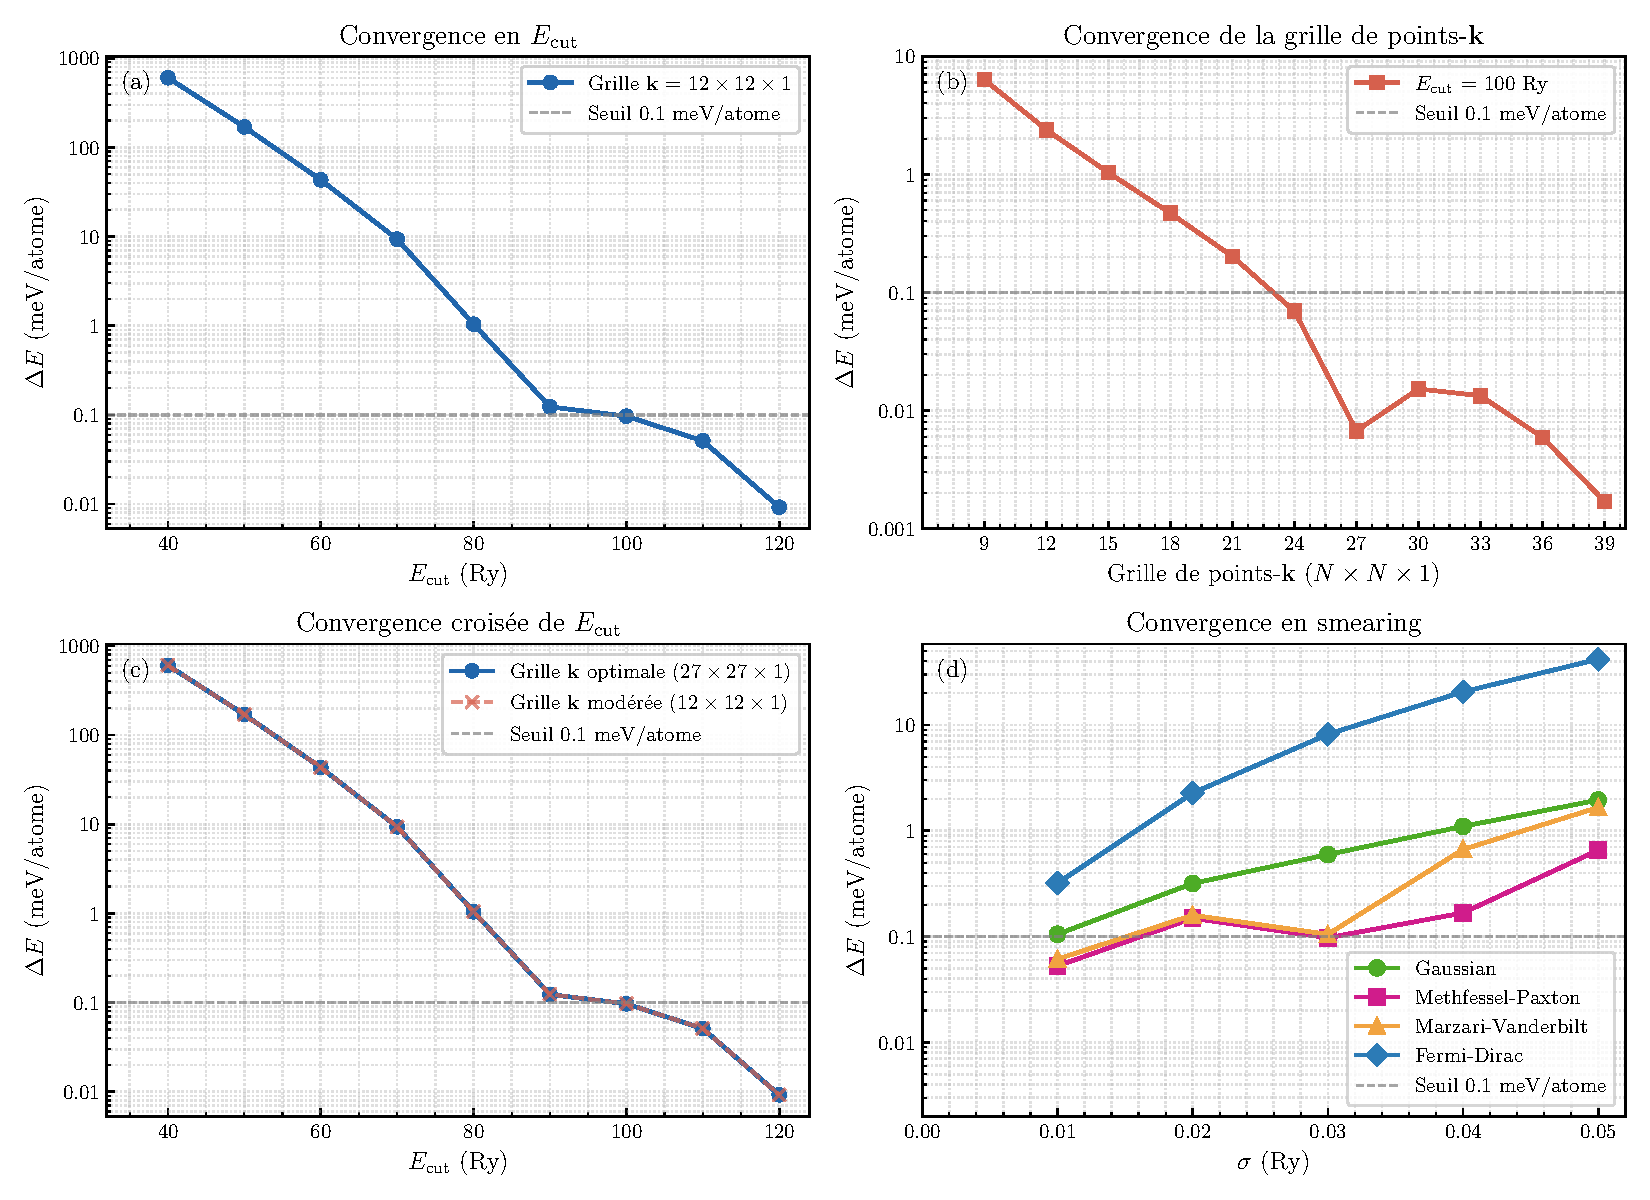
\includegraphics[width=\textwidth]{figures/fig_convergence.pdf}
    \caption[Étude de convergence sur divers paramètres affectant la convergence de l'état fondamental des électrons dans une feuille de graphène parfaite.]{Étude de convergence sur divers paramètres affectant la convergence de l'état fondamental des électrons dans une feuille de graphène parfaite. (a) Étude de convergence sur l'énergie de coupure des ondes planes pour une grille MP de points-$\kv$ modérément dense $12\times12\times1$. (b) Étude de convergence sur la densité de l'échantillonnage de la BZ à l'aide de grilles MP de points-$\kv$ à $E_\text{cut}=100$ Ry optimal. (c) Étude de convergence croisée sur la coupure d'énergie des ondes planes pour la grille MP optimale de $27\times27\times1$. (d) Étude de convergence sur les différents schémas de \textit{smearing} à différentes valeurs de la pseudo-température $\sigma$, calculée avec la grille MP de $27\times27\times1$ optimale et à $E_\text{cut}=100$ Ry optimal. Tous les calculs ont été réalisés avec la fonctionnelle XC PBE et le pseudo-potentiel ONCV \textit{stringent} pour le carbone tiré de la bibliothèque PseudoDojo~\cite{vansettenPseudoDojoTrainingGrading2018}.}
    \label{fig:convergence}
\end{figure}

Premièrement, le test de convergence par rapport à la coupure d'énergie des ondes planes $E_\text{cut}$ pour une grille $\kv$ MP modérément dense de $12\times12\times1$ est illustré à la figure~\ref{fig:convergence} (a). L'énergie totale est variationnelle par rapport à $E_\text{cut}$ et donc on s'attend à une décroissance monotone de l'énergie pour des énergies de coupures croissantes. En observant cette figure, nous voyons bien la décroissance monotone et nous voyons que le premier $E_\text{cut}$ qui tombe sous le seuil de 0.1 meV/atome est $E_\text{cut}=100$ Ry. Nous choisissons donc cette valeur comme étant le $E_\text{cut}$ optimal pour les électrons. Ensuite, nous faisons le test de convergence pour la densité de l'échantillonnage de la BZ, avec $E_\text{cut}$ fixé à sa valeur optimale de 100 Ry, à la figure~\ref{fig:convergence} (b). L'énergie n'est pas variationnelle par rapport à la densité d'échantillonnage, ce qui est reflété dans la figure. Cependant, l'échantillonnage de la BZ a une forte influence sur l'énergie totale : pour les métaux et les semi-métaux, les points-$\kv$ proches du niveau de Fermi contribuent plus à l'énergie, il est donc important de bien échantillonner proche du niveau de Fermi. Pour le graphène, il est critique d'avoir le point $\Kv=(1/3, 1/3, 0)$ dans sa grille, donc des grilles MP qui sont des multiples de 3. En observant la figure~\ref{fig:convergence} (b), nous voyons que la première grille sous le seuil de 0.1 meV/atome est la grille $24\times24\times1$. Malgré cela, nous avons choisi la grille $27\times27\times1$, car elle offre un échantillonnage plus dense proche du niveau Fermi et réduit l'énergie significativement à un coût computationnel légèrement accru. De plus, dans certains systèmes, les convergences pour $E_\text{cut}$ et la grille MP ne sont pas indépendantes. Pour vérifier cela, nous avons un autre test de convergence sur $E_\text{cut}$, cette fois-ci avec la grille MP optimale de $27\times27\times1$. Le résultat se trouve dans la figure~\ref{fig:convergence} (c) et nous pouvons voir que la courbe converge vers la même valeur, confirmant que les deux paramètres sont indépendants dans ce système. Finalement, le test de convergence par rapport aux schémas de \textit{smearing} et le facteur d'élargissement $\sigma$ est présenté dans la figure~\ref{fig:convergence} (d), pour $E_\text{cut}$ et la grille MP fixés à leur valeur optimale. Nous voyons que le \textit{smearing} de Fermi-Dirac est celui qui converge le moins vite et ne descend jamais sous le seuil. Le schéma Gaussien, quant à lui, converge plus vite que Fermi-Dirac, s'approchant du seuil, sans toutefois le franchir. Pour finir, nous voyons que les schémas de Methfessel-Paxton et de Marzari-Vanderbilt sont assez similaires, avec Methfessel-Paxton qui converge marginalement plus vite, et sont les deux significativement meilleurs que les schémas de Fermi-Dirac et Gaussien. Les deux descendent en dessous du seuil pour $\sigma=0.01$ Ry. Nous avons choisi d'utiliser le schéma de Marzari-Vanderbilt avec $\sigma=0.01$ Ry, car contrairement à Methfessel-Paxton, ce schéma reste dans l'intervalle physique $[0,1]$ ce qui est particulièrement important pour la stabilité du cycle SCF et est plus robuste aux perturbations que nous allons inclure dans la feuille de graphène. En résumé, les paramètres optimaux retenus pour l'état fondamental 
des électrons sont $E_\text{cut}=100$ Ry, une grille $\kv$ MP 
$27\times27\times1$ et le \textit{smearing} de Marzari-Vanderbilt 
avec $\sigma=0.01$ Ry.

\begin{figure}[t]
    \centering
    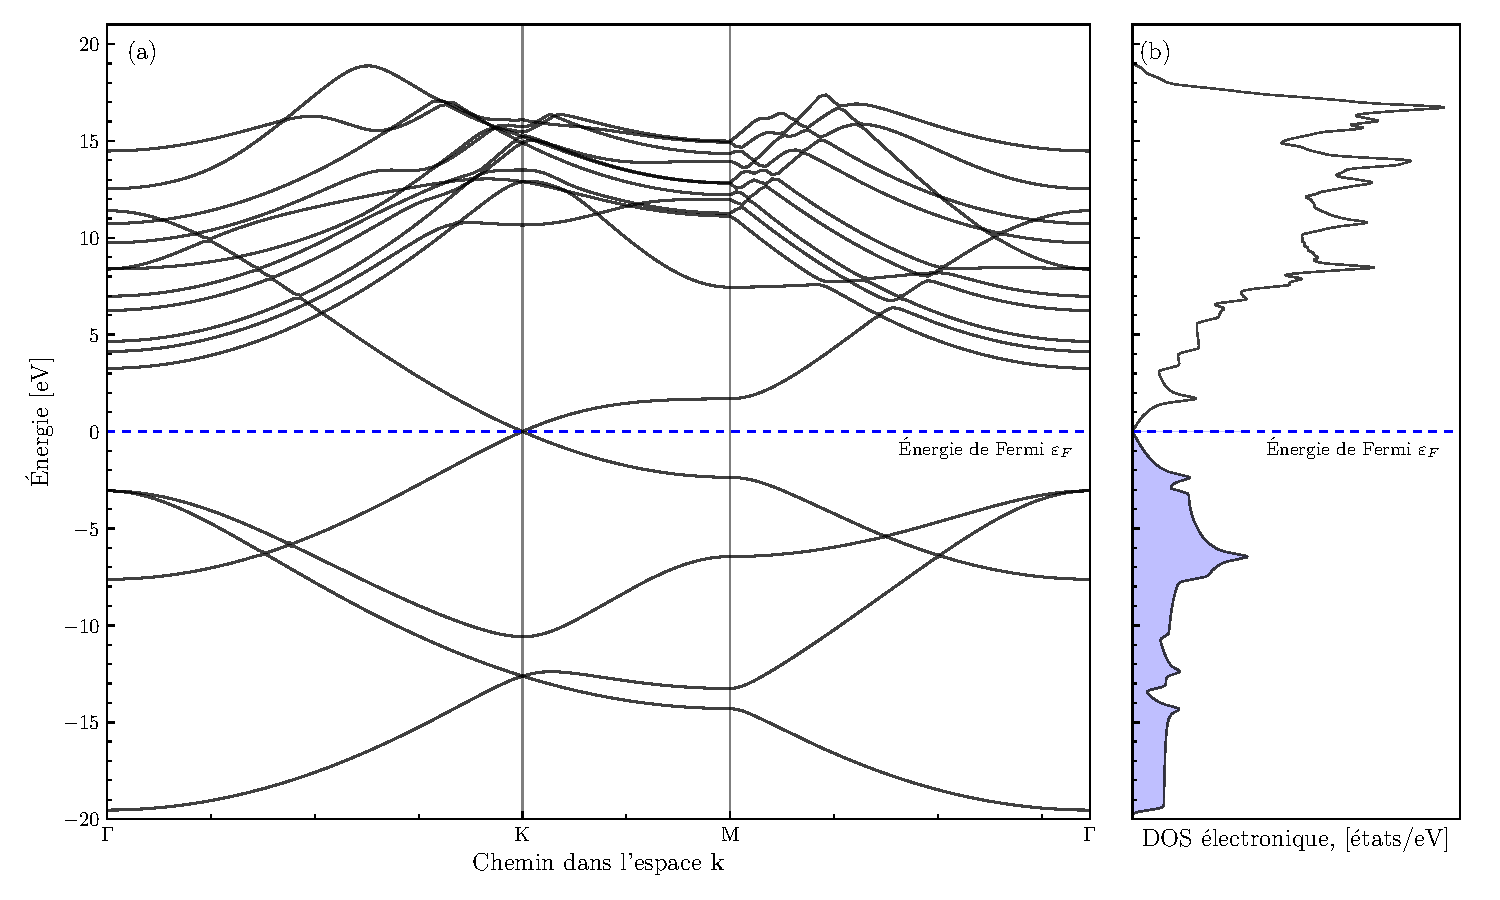
\includegraphics[width=\textwidth]{figures/fig_ebands_edos.pdf}
    \caption[Structure de bandes et densité d'états électronique pour une feuille de graphène parfaite.]{Structure de bandes et densité d'états électronique pour une feuille de graphène parfaite à partir d'un calcul SCF préalable avec les paramètres convergés de la figure~\ref{fig:convergence} : la fonctionnelle XC PBE, le pseudo-potentiel ONCV \textit{stringent} PseudoDojo pour le carbone, $E_\text{cut}=100$ Ry, une grille MP $27\times27\times1$ et du \textit{smearing} MV avec $\sigma=0.01$ Ry. (a) Structure de bandes du graphène parfait calculée le long du chemin $\Gamma\to K\to M\to\Gamma$ de la BZ avec $60$ points par segment. Seules les 16 premières bandes sont illustrées. (b) Densité d'états électronique calculée sur une grille MP plus dense de $96\times96\times1$ et  avec un élargissement Gaussien de $\sigma=0.01$ Ry.}
    \label{fig:resultats_electrons}
\end{figure}

Avec ces paramètres, les équations de KS sont résolues de manière autocohérente pour converger la densité en suivant la prescription de la figure~\ref{fig:scf_PW}. Une fois la densité convergée, le potentiel de KS $V_\text{KS}$ est calculé, puis l'Hamiltonien de KS $H_\text{KS}$ est construit sur n'importe quelle grille ou chemin dans l'espace $\kv$,  puis est diagonalisé une dernière fois pour les valeurs propres $\varepsilon_{n\kv}$ et les fonctions d'onde $\psi_{n\kv}(\rv)$. Les valeurs propres sont tracées en fonction des points$-\kv$ sur un chemin unidimensionnel dans la BZ qui passe par des points d'intérêt de haute symétrie. Les valeurs propres peuvent également être utilisées pour calculer la densité d'états électroniques (DOS, de l'anglais \textit{Density of States})
\begin{equation}
    D(\varepsilon)=\sum_{n\kv}\delta(\varepsilon-\varepsilon_{n\kv})
    \label{eqn:c2_edos}
\end{equation}
qui représente le nombre d'états électroniques par unité d'énergie disponibles à l'énergie $\varepsilon$. En pratique, la fonction delta est remplacée par une Gaussienne avec un facteur d'élargissement $\sigma$, puisqu'il n'est pas possible de représenter une fonction delta numériquement. Ce facteur joue un peu le même rôle que le facteur d'élargissement pour le \textit{smearing}, nous lui attribuons donc le même symbole. Intégrer la DOS sur les états occupés donne le nombre d'électrons dans la cellule unitaire $N_e$:
\begin{equation}
    \int_{-\infty}^{\varepsilon_F}d\varepsilon\,D(\varepsilon)=N_e,
    \label{eqn:c2_dos_int}
\end{equation}
ce qui donne 8 pour le graphène. 

La structure de bandes et la densité d'états électronique pour une feuille de graphène parfaite sont illustrées dans la figure~\ref{fig:resultats_electrons}. La structure de bandes est représentée dans la figure~\ref{fig:resultats_electrons} (a). L'état fondamental a été calculé avec les paramètres donnés plus haut dans cette section, puis l'Hamiltonien a été diagonalisé le long du chemin $\Gamma\to K\to M\to\Gamma$ avec 60 points par segment. Nous voyons les trois bandes $\sigma-sp^2$ plus basses en énergie et la bande $\pi-p_z$ qui touche linéairement la bande $\pi^*-p_z$ au niveau de Fermi et au point $\Kv$ de la BZ. C'est le cône de Dirac. La dispersion linéaire au point de Dirac donne lieu à une vitesse de Fermi $v_F\approx10^6$ m/s~\cite{castronetoElectronicPropertiesGraphene2009,novoselovTwodimensionalGasMassless2005} qui témoigne de la mobilité très élevée des électrons dans le graphène.

La DOS est représentée dans la figure~\ref{fig:resultats_electrons} (b). Elle a été calculée sur une grille MP plus dense de $96\times96\times1$ et un facteur d'élargissement $\sigma=0.01$ Ry a été utilisé. La partie colorée représente les états occupés et nous voyons bien que la densité d'états est nulle à l'énergie de Fermi, ce qui confirme que le graphène parfait est un semi-métal avec un gap nul au point de Dirac à température nulle. Pour toute température $T>0$, l'agitation thermique peuple continuellement la bande $\pi^*$, ce qui explique que le graphène est conducteur à température finie. Nous voyons également que les singularités de Van Hove~\cite{dresselhausPhysicalPropertiesCarbon1998,BassaniParraviciniElectronic} (les pics dans la DOS aux points d'inflexion de la structure de bandes au point $\mathbf{M}$) sont bien reproduites. Ces résultats sont en excellent accord avec les calculs DFT-PBE de la littérature~\cite{castronetoElectronicPropertiesGraphene2009}.

\section{Partie ionique : les phonons et la théorie de la fonctionnelle de la densité perturbative}\label{sec:phonons}
À l'instar de son homologue électronique, le problème ionique n'est pas moins complexe à résoudre que le problème initial. Le coupable est encore une fois l'interaction mutuelle entre tous les ions qui se trouve dans le potentiel effectif $U$. Ce problème est toutefois plus accessible que le problème électronique, car les ions sont beaucoup plus massifs que les électrons, ce qui confine leur fonction d'onde à des régions très localisées autour de leur position d'équilibre\footnote{Ce raisonnement ne s'applique pas aux ions les plus légers du tableau périodique comme l'hydrogène.}. Cette localisation permet de traiter les ions semi-classiquement et leur dynamique est gouvernée par les équations de Newton. Cependant, la spectroscopie Raman implique des processus d'émission et d'absorption de quanta d'énergie vibrationnelle qui nécessitent une description quantique. Dans cette section, nous résolvons le problème ionique avec une approche semi-classique dans l'approximation harmonique, puis nous quantifions les vibrations des ions pour avoir une théorie quantique. Nous présentons aussi brièvement le couplage entre les électrons et les quanta de vibrations des ions : le couplage électron-phonon, indispensable pour la spectroscopie Raman. Finalement, nous présentons nos résultats des propriétés vibrationnelles du graphène parfait.

\subsection{Approximation harmonique}\label{sec:harmonique}
Une fois que le problème électronique est résolu avec \textit{e.g.} la DFT, nous permettons aux ions de bouger, ou plus précisément d'osciller autour de leur position d'équilibre. Pour décrire les positions ioniques, nous utilisons un indice composé $I=l\alpha$, où $l$ identifie la cellule unitaire située à $\Rv_l$ et $\alpha$ indexe les ions situés à $\bm{\tau}_\alpha$ dans la cellule unitaire, de sorte que leur position s'écrit maintenant
\begin{equation}
    \rv_{l\alpha}=\Rv_l+\bm{\tau}_\alpha+\mathbf{u}_{\ell\alpha},
    \label{eqn:c2_rla}
\end{equation}
où $\mathbf{u}_{l\alpha}$ est le déplacement autour de l'équilibre de l'ion $\alpha$ dans la cellule $l$. Avec cette notation, le problème à résoudre est maintenant
\begin{equation}
    \hat{H}_i=-\sum_{l\alpha}\frac{\hbar^2}{2M_\alpha}\nabla^2_{\rv_{l\alpha}}+U.
    \label{eqn:c2_Hila}
\end{equation}
Le potentiel effectif $U$ contient le couplage entre tous les ions et l'énergie de l'état fondamental des électrons. Pour contourner les difficultés qui lui sont associées, il est utile de supposer que les déplacements des ions $\mathbf{u}_{l\alpha}$ sont petits et de faire l'expansion en série de Taylor du potentiel autour de la position d'équilibre et de tronquer après le deuxième ordre
\begin{equation}
    U\approx \frac{1}{2}\sum_{l\alpha\mu}\sum_{l'\alpha'\mu'}C_{l\alpha\mu,l'\alpha'\mu'}u_{l\alpha\mu}u_{l'\alpha'\mu'},
\end{equation}
où $\mu=x,y,z$ dénote les composantes des vecteurs. Le terme d'ordre zéro n'est qu'une constante et a été ignoré. Le terme de premier ordre, qui est la dérivée du potentiel à l'équilibre, est proportionnel à la force exercée sur les ions, qui est nulle par définition à l'équilibre. Dans le terme de deuxième ordre, nous avons défini la matrice des constantes de force interatomiques (IFC, de l'anglais \textit{Interatomic Force Constants})
\begin{equation}
    C_{l\alpha\mu,l'\alpha'\mu'}\equiv \frac{\partial^2U}{\partial u_{l\alpha\mu}\partial u_{l'\alpha'\mu'}}\bigg\rvert_{\mathbf{u}=\mathbf{0}}.
    \label{eqn:c2_IFC}
\end{equation}
Tronquer la série après le deuxième ordre donne lieu à l'approximation harmonique, qui remplace l'interaction mutuelle complexe par une interaction beaucoup plus simple où chaque ion est vu comme étant relié à tous les autres par des ressorts de constantes de rappel données par les IFCs. Nous voulons résoudre pour les déplacements des ions $u_{l\alpha\mu}$. Pour ce faire, nous pouvons utiliser la deuxième loi de Newton
\begin{equation}
    F_{l\alpha\mu}=M_\alpha \frac{\partial ^2 u_{l\alpha\mu}}{\partial t^2}=-\frac{\partial U}{\partial u_{l\alpha\mu}},
\end{equation}
d'où la description semi-classique. En supposant des déplacements sous forme d'ondes planes, justifiée par l'approximation harmonique, $u_{l\alpha\mu}=u_{\alpha\mu}(\qv)e^{i(\qv\cdot\Rv_l-\omega t)}$, nous obtenons les équations de mouvement pour les ions
\begin{equation}
    \omega_{\nu\qv}^2e_{\alpha\mu}^{(\nu)}(\qv)=\sum_{\alpha'\mu'}D_{\alpha\mu,\alpha'\mu'}(\qv)e_{\alpha'\mu'}^{(\nu)}(\qv).
    \label{eqn:c2_ionsEOM}
\end{equation}
Ici, nous avons défini la matrice dynamique, qui est reliée à la transformée de Fourier de la matrice des IFCs
\begin{equation}
    D_{\alpha\mu,\alpha'\mu'}(\qv)\equiv\frac{1}{\sqrt{M_\alpha M_{\alpha'}}}\sum_{\Rv_l}C_{\alpha\mu,\alpha'\mu'}(\Rv_l)e^{i\qv\cdot\Rv_l},
    \label{eqn:c2_D}
\end{equation}
et les déplacements pondérés en masse $e_{\alpha\mu}^{(\nu)}(\qv) = \sqrt{M_\alpha}u_{\alpha\mu}(\qv)$. L'équation \eqref{eqn:c2_ionsEOM} est une équation aux valeurs propres pour les fréquences de phonon $\omega_{\nu\qv}$ et les modes normaux des déplacements $e_{\alpha\mu}^{(\nu)}(\qv)$. Pour un système avec $p$ ions dans la cellule unitaire, la matrice dynamique est une matrice $3p\times 3p$ et nous utilisons l'indice $\nu=1,\dots,3p$ pour étiqueter les $3p$ valeurs et modes normaux. Cet indice, l'indice de branche, joue un rôle analogue à l'indice de bande $n$ des électrons.

La description semi-classique de l'approximation harmonique donne 
accès aux fréquences de vibration $\omega_{\nu\qv}$ et aux modes 
normaux $e_{\alpha\mu}^{(\nu)}(\qv)$, mais ne suffit pas pour 
décrire les propriétés quantiques des vibrations du réseau. En 
effet, les expériences montrent que les vibrations n'échangent 
de l'énergie qu'en paquets discrets $\hbar\omega_{\nu\qv}$ avec 
la lumière et les électrons --- une propriété fondamentalement 
quantique. De plus, la spectroscopie Raman, au cœur de ce 
mémoire, est un processus de création et d'annihilation de 
quasiparticules vibrationnelles, ce qui nécessite une description 
quantique. Il est donc nécessaire de quantifier les vibrations 
du réseau, ce que nous faisons dans la prochaine section.

\subsection{Quantification des vibrations du réseau : phonons}

Dans l'approximation harmonique, l'Hamiltonien des ions prend la forme plus simple
\begin{equation}
    \hat{H}_i = \sum_{l\alpha\mu}\frac{p_{l\alpha\mu}^2}{2M_\alpha}+\frac{1}{2}\sum_{l\alpha\mu}\sum_{l'\alpha'\mu'}C_{l\alpha\mu,l'\alpha'\mu'}u_{l\alpha\mu}u_{l'\alpha'\mu'}.
\end{equation}
En utilisant le développement des déplacements atomiques en combinaison linéaire des modes normaux et son équivalent pour le moment conjugué $p_{l\alpha\mu}=M_\alpha\dot{u}_{l\alpha\mu}$, nous obtenons l'Hamiltonien dans l'espace réciproque
\begin{equation}
    \hat{H}_i = \frac{1}{2}\sum_{\nu\qv}\left(\dot{Q}_{\nu\qv}\dot{Q}_{\nu-\qv}+\omega_{\nu\qv}^2Q_{\nu\qv}Q_{\nu-\qv}\right),
\end{equation}
qui est une somme d'oscillateurs harmoniques. La quantification des vibrations des ions suit la procédure standard de la quantification canonique : les coordonnées normales $Q_{\nu\qv}$ et leurs moments conjugués $P_{\nu\qv}=\dot{Q}_{\nu\qv}$ sont promus au rang d'opérateurs quantiques satisfaisant les relations de commutation canoniques
\begin{equation}
    [\hat{Q}_{\nu\qv},\hat{P}_{\nu'\qv'}]=i\hbar\delta_{\nu\nu'}\delta_{\qv\qv'}.
\end{equation}
Ensuite, de manière analogue à l'oscillateur harmonique quantique simple, nous introduisons les opérateurs de création $\hat{b}^\dag_{\nu\qv}$ et d'annihilation $\hat{b}_{\nu\qv}$
\begin{equation}
    \hat{b}_{\nu\qv}=\sqrt{\frac{\omega_{\nu\qv}}{2\hbar}}\left(\hat{Q}_{\nu\qv}+\frac{i}{\omega_{\nu\qv}}\hat{P}_{\nu\qv}\right),
\end{equation}
avec $\hat{b}^\dag_{\nu\qv}=(\hat{b}_{\nu\qv})^\dag$ et où $\hat{b}^\dag_{\nu\bv}\,(\hat{b}_{\nu\qv})$ crée (détruit) une quasiparticule dans la branche $\nu$ avec un vecteur d'onde $\qv$. Ces quasiparticules associées aux excitations des vibrations des ions sont les \textit{phonons}. Un phonon dans la branche $\nu$ et avec un vecteur d'onde $\qv$ a une énergie $\hbar\omega_{\nu\qv}$ et un quasi-moment $\hbar\qv$. Avec cette transformation canonique, l'Hamiltonien harmonique prend la forme élégante
\begin{equation}
    \hat{H}_\text{ph}=\sum_{\nu\qv}\hbar\omega_{\nu\qv}\left(\hat{b}_{\nu\qv}^\dag \hat{b}_{\nu\qv}+\frac{1}{2}\right).
\end{equation}
qui est l'Hamiltonien des phonons libres. Les opérateurs de phonons satisfont les relations de commutation bosoniques de sorte qu'ils obéissent à la statistique de Bose-Einstein et que leur nombre d'occupation moyen à température $T$ est donné par la distribution de Bose-Einstein
\begin{equation}
    \langle \hat{n}_{\nu\qv}\rangle =\frac{1}{e^{\hbar\omega_{\nu\qv}/k_BT}-1},
\end{equation}
où $\hat{n}_{\nu\qv}=\hat{b}^\dag_{\nu\qv}\hat{b}_{\nu\qv}$. Finalement, les équations pour les opérateurs de phonons peuvent être inversées pour écrire les coordonnées normales en termes des opérateurs de phonons
\begin{align}
    \hat{Q}_{\nu\qv}&=\sqrt{\frac{\hbar}{2\omega_{\nu\qv}}}\hat{A}_{\nu\qv}\label{eqn:c2_Qn},\\
    \hat{A}_{\nu\qv}&=\hat{b}_{\nu\qv}+\hat{b}_{\nu-\qv}^\dag,\label{eqn:c2_An}
\end{align}
où nous avons défini l'opérateur $\hat{A}_{\nu\qv}$ qui est proportionnel au mode de déplacement et qui nous sera utile lorsque nous discuterons du couplage entre les électrons et les phonons au chapitre \ref{chap:eph}.

Les phonons sont donc complètement caractérisés par leur vecteur d'onde $\qv$, leur branche $\nu$, leur fréquence $\omega_{\nu\qv}$ et leur vecteur de polarisation $\mathbf{e}^{(\nu)}(\qv)$. Pour obtenir ces quantités, il est nécessaire de calculer la matrice dynamique $D_{\alpha\mu,\alpha'\mu'}(\qv)$ (équation~\eqref{eqn:c2_D}), qui requiert à son tour le calcul de la matrice des IFCs $C_{\ell\alpha\mu,\ell'\alpha'\mu'}$ (équation~\eqref{eqn:c2_IFC}). Il existe deux approches principales pour calculer les IFCs à partir des premiers principes. La première est la méthode des phonons gelés (\textit{frozen phonons}), qui consiste à déplacer légèrement les ions autour de leur position d'équilibre et à calculer numériquement les dérivées via un schéma de différence finie. Cette méthode est conceptuellement simple à implémenter, mais nécessite un calcul SCF complet pour chaque déplacement et est limitée aux vecteurs $\qv$ commensurables avec la supercellule utilisée, ce qui rend les calculs coûteux. La deuxième approche, plus élégante et plus efficace, est de calculer les deuxièmes dérivées à l'aide de la théorie de la perturbation en mécanique quantique dans le cadre de la DFT : la théorie de la fonctionnelle de la densité perturbative (DFPT), que nous présentons dans la prochaine section.

\subsection{Théorie de la fonctionnelle de la densité perturbative}\label{sec:dfpt}
L'idée centrale est de considérer les vibrations ioniques --- les phonons --- comme une perturbation externe sur les électrons et d'effectuer des calculs de théorie de la perturbation dans le cadre de la DFT, une méthode qui se nomme théorie de la fonctionnelle de la densité perturbative (DFPT)~\cite{baroniPhononsRelatedCrystal2001a,baroniGreensfunctionApproachLinear1987,gonzeDensityfunctionalApproachNonlinearresponse1989,savrasovLinearresponseTheoryLattice1996}. La DFPT fut développée au cours des années 1990 et s'applique à n'importe quelle perturbation externe sur les électrons, faisant d'elle une méthode très générale. Dans cette section nous voyons brièvement les bases de la théorie de la perturbation dans le cadre de la DFT et de son application aux phonons.

\noindent\textbf{Perturbation générale}

Dans la théorie de la perturbation en mécanique quantique, il est supposé que la perturbation est caractérisée par un paramètre continu $\lambda\ll1$ et que nous pouvons faire l'expansion d'une quantité du système $X$ en série de Taylor
\begin{equation}
    X(\lambda)=X^{(0)}+\lambda X^{(1)}+\frac{\lambda^2}{2!}X^{(2)}+\dots,\label{eqn:c2_X}
\end{equation}
où $X^{(0)}$ est la quantité $X$ en l'absence de la perturbation  et $X^{(n)}$ sont les corrections d'ordre $n=1,2,\dots$ à $X^{(0)}$ dues à la perturbation. Comme c'est une expansion en série de Taylor, nous avons que
\begin{equation}
    X^{(n)}=\frac{\partial^n X}{\partial\lambda^n}\bigg\rvert_{\lambda=0}.\label{eqn:c2_Xn}
\end{equation}
Cette méthode est particulièrement efficace lorsque la perturbation est petite par rapport aux énergies caractéristiques du système, soit quand $\lambda$ est petit, et qu'il est possible de tronquer l'expansion de l'équation~\eqref{eqn:c2_X} après le premier ou le deuxième ordre.

Pour des électrons en interaction traités dans le cadre de la DFT, les quantités $X$ qui nous intéressent sont l'Hamiltonien de KS $\hat{H}_\text{KS}$, les valeurs propres de KS $\varepsilon_{n\kv}$, les fonctions d'onde de KS $\ket{\psi_{n\kv}}$ ainsi que la densité $n(\rv)$. Nous avons déjà résolu le problème pour le système en absence de perturbation, ce n'est que l'équation de KS pour le système non-perturbé
\begin{equation}
    \hat{H}_\text{KS}^{(0)}\ket{\psi_{n\kv}^{(0)}}=\varepsilon_{n\kv}^{(0)}\ket{\psi_{n\kv}^{(0)}}.
    \label{eqn:c2_KSnonperturbe}
\end{equation}
Le théorème $2n+1$~\cite{dalgarnoPerturbationCalculationProperties1958,gonzeDensityfunctionalApproachNonlinearresponse1989,gonzeAdiabaticDensityfunctionalPerturbation1995,baroniPhononsRelatedCrystal2001a} stipule que pour obtenir la correction d'ordre $2n+1$ à l'énergie totale (donc la dérivée d'ordre $2n+1$), seules les corrections d'ordre $n$ aux fonctions d'onde sont nécessaires. 
Dans le contexte d'une perturbation due à des phonons, pour calculer la matrice IFC, qui est une deuxième dérivée de l'énergie totale, nous n'avons besoin que de la correction de premier ordre aux fonctions d'onde. Pour la trouver, il faut considérer l'équation de KS pour le système perturbé
\begin{equation}
    \hat{H}_\text{KS}\ket{\psi_{n\kv}}=\varepsilon_{n\kv}\ket{\psi_{n\kv}}
\end{equation}
et faire l'expansion des quantités présentes en utilisant l'expansion de l'équation~\eqref{eqn:c2_X}. En ne retenant que les termes proportionnels à $\lambda$ et en utilisant l'équation de KS non-perturbée (équation~\eqref{eqn:c2_KSnonperturbe}), nous obtenons la célèbre équation de Sternheimer~\cite{gonzeAdiabaticDensityfunctionalPerturbation1995}
\begin{equation}
    \left(\hat{H}^{(0)}_\text{KS}-\varepsilon_{n\kv}^{(0)}\right)\ket{\psi_{n\kv}^{(1)}}=-\left(\hat{H}^{(1)}_\text{KS}-\varepsilon^{(1)}_{n\kv}\right)\ket{\psi^{(0)}_{n\kv}},
    \label{eqn:c2_sternheimer}
\end{equation}
sujette à la contrainte de normalisation $\bra{\psi_{n\kv}^{(0)}}\ket{\psi_{n\kv}^{(1)}}=0$. L'opérateur $\hat{H}^{(0)}_\text{KS}-\varepsilon_{n\kv}^{(0)}$ n'est pas inversible, puisqu'il a $\ket{\psi_{n\kv}^{(0)}}$ comme état propre de valeur propre nulle. La solution $\ket{\psi_{n\kv}^{(1)}}$ n'est donc définie qu'à une composante parallèle à $\ket{\psi_{n\kv}^{(0)}}$ près. Cette composante est précisément fixée par le choix de normalisation $\bra{\psi_{n\kv}^{(0)}}\ket{\psi_{n\kv}^{(1)}}=0$ : seule la projection de $\ket{\psi_{n\kv}^{(1)}}$ sur l'espace des états vides est inconnue. Pour exploiter ce fait, nous introduisons le projecteur sur les états vides (de conduction):
\begin{equation}
    \hat{P}_c = 1-\hat{P}_v = 1-\sum_{m}f_{m\kv}\ket{\psi_{m\kv}^{(0)}}\bra{\psi_{m\kv}^{(0)}}.
\end{equation}
En appliquant $\hat{P}_c$ sur l'équation de Sternheimer~\eqref{eqn:c2_sternheimer} en notant que $\hat{P}_c\ket{\psi_{n\kv}^{(0)}}=0$ annihile le terme en $\varepsilon_{n\kv}^{(1)}$, nous obtenons la forme effectivement résolue en pratique de l'équation de Sternheimer
\begin{equation}
    \left(\hat{H}^{(0)}_\text{KS}-\varepsilon_{n\kv}^{(0)}\right)\ket{\psi_{n\kv}^{(1)}}=- \hat{P}_c \hat{H}_{\text{KS}}^{(1)}\ket{\psi_{n\kv}^{(0)}}.
    \label{eqn:c2_sternheimer_proj}
\end{equation} 
Sous cette forme, l'opérateur du membre de gauche, restreint à l'espace vide, est non-singulier et inversible par une méthode itérative. Surtout, la correction à la fonction d'onde $\ket{\psi_{n\kv}^{(1)}}$ s'obtient sans jamais évaluer explicitement la somme sur les états non-occupés ni la correction à l'énergie $\varepsilon_{n\kv}^{(1)}$. C'est un avantage considérable de la DFPT par rapport à la théorie de la perturbation par somme sur les états ordinaire et qui rend la DFPT pratiquable à des systèmes comportant un grand nombre de bandes~\cite{baroniPhononsRelatedCrystal2001a}. 

La correction de premier ordre à la fonction d'onde s'obtient donc en résolvant l'équation de Sternheimer projetée~\eqref{eqn:c2_sternheimer_proj}, pourvu que nous connaissions la correction de premier ordre à l'Hamiltonien $H_\text{KS}^{(1)}$. Cette dernière s'obtient en prenant la dérivée de l'Hamiltonien par rapport à la perturbation~\eqref{eqn:c2_Xn}. Dans l'Hamiltonien de KS perturbé, le potentiel externe dépend directement de la perturbation, tandis que les potentiels d'Hartree et d'échange-corrélation dépendent implicitement de la perturbation au travers de la densité :
\begin{equation}
    \hat{H}_\text{KS}^{(1)}=\frac{\partial \hat{H}_\text{KS}}{\partial \lambda}\bigg\rvert_{\lambda=0}=\frac{\partial V_\text{ext}}{\partial\lambda}\bigg\rvert_{\lambda=0}+\int d^3\rv'\,\frac{\delta V_\text{H}(\rv)}{\delta n(\rv')}n^{(1)}(\rv')+\int d^3\rv'\,\frac{\delta V_\text{XC}(\rv)}{\delta n(\rv')}n^{(1)}(\rv'),
    \label{eqn:c2_H1}
\end{equation} 
où $n^{(1)}(\rv)=\partial n(\rv)/\partial \lambda$ est la correction de premier ordre à la densité due à la perturbation. Pour la trouver, il suffit de partir de l'équation pour la densité~\eqref{eqn:c2_nKS}
\begin{equation}
    n(\rv)=2\sum_{n\kv}f_{n\kv}\psi^*_{n\kv}(\rv)\psi_{n\kv}(\rv),
\end{equation}
de faire l'expansion~\eqref{eqn:c2_X} des fonctions d'onde et de ne conserver que les termes proportionnels à $\lambda$, pour obtenir
\begin{equation}
    n^{(1)}(\rv)=4\Re\sum_{n\kv}f_{n\kv}\psi_{n\kv}^{*{(0)}}(\rv)\psi_{n\kv}^{(1)}(\rv).
    \label{eqn:c2_n1}
\end{equation}

Les équations \eqref{eqn:c2_sternheimer_proj}-\eqref{eqn:c2_H1}-\eqref{eqn:c2_n1} forment un ensemble d'équations autocohérentes à résoudre pour la correction de premier ordre à la fonction d'onde. Pour la trouver, il faut résoudre l'équation de Sternheimer projetée~\eqref{eqn:c2_sternheimer_proj}. Pour résoudre cette équation, nous avons besoin de la correction au premier ordre de l'Hamiltonien, qui s'obtient en résolvant l'équation~\eqref{eqn:c2_H1}. Pour résoudre cette dernière, il faut la correction de premier ordre à la densité en résolvant l'équation~\eqref{eqn:c2_n1}, pour laquelle nous avons besoin de la correction de premier ordre à la fonction d'onde, la quantité recherchée initialement. La résolution de ce cycle admet une forme similaire au cycle SCF de la DFT classique.

\noindent\textbf{Perturbation par vibration ionique}

Nous avons traité jusqu'ici d'une perturbation générale paramétrée par $\lambda$. Nous spécialisons maintenant ce formalisme au cas qui nous intéresse, celui où la perturbation est le déplacement des ions hors de leur position d'équilibre -- les phonons. La position de l'ion $\alpha$ dans la cellule $l$ s'écrit $\rv_{l\alpha}=\Rv_l +\bm{\tau}_{\alpha}+\mathbf{u}_{l\alpha}$. Ce sont les composantes cartésiennes $u_{l\alpha\mu}$ ($\mu=x,y,z$) du déplacement qui jouent désormais le rôle du paramètre $\lambda$. Parmi les termes de l'Hamiltonien de Kohn-Sham, seul le potentiel externe (qui est remplacé par un pseudo-potentiel, \textit{c.f.} la section~\ref{sec:PP}) dépend explicitement des déplacements ioniques. Les potentiels d'Hartree et d'échange-corrélation n'en dépendent qu'implicitement, au travers de la densité.

Le déplacement d'un ion brise la symétrie de translation discrète du solide, rendant le théorème de Bloch invalide. Une approche directe exigerait de travailler dans une supercellule suffisamment grande pour contenir la perturbation : c'est la méthode des phonons gelés (\emph{frozen phonon}). Cette approche est coûteuse numériquement et ne donne accès qu'aux phonons dont la longueur d'onde est commensurable avec la supercellule employée. La DFPT contourne ces difficultés en exploitant le caractère ondulatoire des vibrations. Pour $p$ atomes dans la cellule unitaire, nous appliquons $3p$ perturbations de la forme
\begin{equation}
    u_{l\alpha\mu}(\qv)=u_{\alpha\mu}e^{i\qv\cdot \Rv_l}.
\end{equation}
Pour chaque perturbation élémentaire $(\qv,\alpha,\mu)$, nous définissons la dérivée du potentiel externe par rapport au déplacement collectif comme la transformée de Fourier de la dérivée par rapport au déplacement d'un ion individuel
\begin{equation}
    \Delta_{\qv\alpha\mu}V_\text{PP}(\rv)\equiv\sum_{l}\frac{\partial V_\text{PP}^{(\alpha)}}{\partial u_{l\alpha\mu}}e^{i\qv\cdot\Rv_l}.
\end{equation}
Pour un pseudo-potentiel avec une partie locale et une partie non-locale séparable, les deux contributions se traitent séparément. La correction à la fonction d'onde induite par ce mode, notée $\Delta_{\qv\alpha\mu}\psi_{n\kv}$, s'obtient en résolvant l'équation de Sternheimer projetée~\eqref{eqn:c2_sternheimer_proj}
\begin{equation}
    \left(\hat{H}^{(0)}_\text{KS}-\varepsilon_{n\kv}^{(0)}\right)\ket{\Delta_{\qv\alpha\mu}\psi_{n\kv}}=-\hat{P}_c\Delta_{\qv\alpha\mu}\hat{H}_\text{KS}\ket{\psi_{n\kv}^{(0)}},
    \label{eqn:c2_Sternheimer_phonon}
\end{equation}
où la correction à l'Hamiltonien est donnée par 
\begin{equation}
    \Delta_{\qv\alpha\mu}\hat{H}_\text{KS} =\Delta_{\qv\alpha\mu} V_\text{PP}+\int d^3\rv'\,\Delta_{\qv\alpha\mu}n(\rv')\frac{\delta V_\text{H}(\rv)}{\delta n(\rv')}+\int d^3\rv'\,\Delta_{\qv\alpha\mu}n(\rv')\frac{\delta V_\text{XC}(\rv)}{\delta n(\rv')}.
    \label{eqn:c2_H1_phonon}
\end{equation}
La correction à la densité s'en déduit par
\begin{equation}
    \Delta_{\qv\alpha\mu}n(\rv)=4\Re\sum_{n\kv}f_{n\kv}\psi^{*(0)}_{n\kv}(\rv)\Delta_{\qv\alpha\mu}\psi_{n\kv}(\rv),
    \label{eqn:c2_n1_phonon}
\end{equation}
Ces trois dernières équations (équations~\eqref{eqn:c2_Sternheimer_phonon}--\eqref{eqn:c2_n1_phonon}) sont à résoudre de manière autocohérente en suivant le cycle SCF de la section précédente.

Une fois le cycle convergé, nous disposons de $\Delta_{\qv\alpha\mu}n$ et $\ket{\Delta_{\qv\alpha\mu}\psi_{n\kv}}$ et l'objectif est de calculer les constantes de force interatomiques, définies par la dérivée seconde de l'énergie totale par rapport aux déplacements~\eqref{eqn:c2_IFC}. Dans l'espace réciproque, l'élément $(\alpha\mu,\alpha'\mu')$ de la matrice des constantes de force au vecteur $\qv$ est
\begin{equation}
        \widetilde{C}_{\alpha\mu,\alpha'\mu'}(\qv)
    =\frac{\partial^2 U}
    {\partial u_{\alpha\mu}(\qv)\,\partial u_{\alpha'\mu'}(\qv)} = \widetilde{C}^{\text{el}}_{\alpha\mu,\alpha'\mu'}(\qv)+\widetilde{C}^{\text{ion}}_{\alpha\mu,\alpha'\mu'}(\qv).
    \label{eqn:c2_IFCq}
\end{equation}
Les constantes de force se séparent en deux parties puisque le potentiel effectif ionique $U$ est la somme de l'énergie de l'état fondamental électronique et de l'énergie d'interaction électrostatique entre les ions. La partie électronique s'obtient en faisant les dérivées de l'énergie de l'état fondamental électronique $E_e$ à l'aide du théorème de Hellmann-Feynman~\cite{EinfuhrungQuantenchemieHellmann1941,feynmanForcesMolecules1939} en notant que seul le potentiel externe dû au pseudo-potentiel dépend explicitement des déplacements ioniques
\begin{equation}
    \widetilde{C}^\text{el}_{\alpha\mu,\alpha'\mu'}(\qv)= \int d^3\rv\,\Delta_{\qv\alpha\mu}n(\rv)\Delta_{\qv\alpha'\mu'}V_\text{PP}(\rv)+\int d^3\rv\,n^{(0)}(\rv)\Delta_{\qv\alpha\mu}\Delta_{\qv\alpha'\mu'}V_\text{PP}(\rv).
\end{equation}
La partie ionique, $\widetilde{C}^{\text{ion}}_{\alpha\mu,\alpha'\mu'}(\qv)$ est la dérivée seconde de l'énergie d'interaction Coulombienne ion-ion par rapport aux déplacements ioniques. Cette contribution est évaluée analytiquement par la méthode d'Ewald~\cite{ewaldBerechnungOptischerUnd1921} et ne dépend pas de la réponse électronique. 

Une fois la matrice des constantes de force construite, la matrice dynamique s'obtient selon l'équation~\eqref{eqn:c2_D}
\begin{equation}
    D_{\alpha\mu,\alpha'\mu'}(\qv)=\frac{1}{\sqrt{M_\alpha M_{\alpha'}}}\widetilde{C}_{\alpha\mu,\alpha'\mu'}(\qv),
\end{equation}
et les fréquences de phonons ainsi que leur polarisation s'obtiennent en diagonalisant la matrice dynamique
\begin{equation}
    \sum_{\alpha'\mu'}D_{\alpha\mu,\alpha'\mu'}(\qv)e_{\alpha'\mu'}^{(\nu)}(\qv)=\omega^2_{\nu\qv}e_{\alpha\mu}^{(\nu)}(\qv).
\end{equation}
La procédure complète de calcul des phonons par DFPT se résume 
ainsi. Pour chaque vecteur $\qv$ de la grille et chaque perturbation 
élémentaire $(\alpha,\mu)$~:
\begin{enumerate}
    \item Partir des fonctions d'onde et de la densité non-perturbées 
    $\ket{\psi_{n\kv}^{(0)}}$ et $n^{(0)}$, solutions du cycle SCF 
    non-perturbé, et initialiser la correction à la densité à 
    $\Delta_{\qv\alpha\mu}n_\text{in}=0$.

    \item Construire la correction à l'Hamiltonien 
    $\Delta_{\qv\alpha\mu}H_\text{KS}$ via 
    l'équation~\eqref{eqn:c2_H1_phonon}
    \[\Delta_{\qv\alpha\mu}\hat{H}_\text{KS} = 
    \Delta_{\qv\alpha\mu}V_\text{PP}
    +\int d^3\rv'\,
    \frac{\delta V_\text{H}(\rv)}{\delta n(\rv')}
    \,\Delta_{\qv\alpha\mu}n(\rv')
    +\int d^3\rv'\,
    \frac{\delta V_\text{XC}(\rv)}{\delta n(\rv')}
    \,\Delta_{\qv\alpha\mu}n(\rv').\]
    Au premier passage, $\Delta_{\qv\alpha\mu}n_\text{in}=0$ et l'on a 
    simplement $\Delta_{\qv\alpha\mu}H_\text{KS}=
    \Delta_{\qv\alpha\mu}V_\text{PP}$.

    \item Résoudre l'équation de Sternheimer 
    projetée~\eqref{eqn:c2_Sternheimer_phonon}
    \[\left(\hat{H}^{(0)}_\text{KS}-\varepsilon_{n\kv}^{(0)}\right)
    \ket{\Delta_{\qv\alpha\mu}\psi_{n\kv}}=
    -\hat{P}_c\,\Delta_{\qv\alpha\mu}\hat{H}_\text{KS}
    \ket{\psi_{n\kv}^{(0)}}\]
    pour tous les états occupés $n\kv$, afin d'obtenir les 
    corrections aux fonctions d'onde 
    $\ket{\Delta_{\qv\alpha\mu}\psi_{n\kv}}$.

    \item Calculer la correction à la densité 
    $\Delta_{\qv\alpha\mu}n_\text{out}$ via 
    l'équation~\eqref{eqn:c2_n1_phonon}
    \[\Delta_{\qv\alpha\mu}n_\text{out}(\rv)=
    4\Re\sum_{n\kv}f_{n\kv}
    \psi^{*(0)}_{n\kv}(\rv)
    \Delta_{\qv\alpha\mu}\psi_{n\kv}(\rv).\]

    \item Si la différence entre $\Delta_{\qv\alpha\mu}n_\text{in}$ 
    et $\Delta_{\qv\alpha\mu}n_\text{out}$ est inférieure à une 
    tolérance spécifiée, le cycle a convergé : passer à l'étape~6. 
    Sinon, mélanger $\Delta_{\qv\alpha\mu}n_\text{in}$ et 
    $\Delta_{\qv\alpha\mu}n_\text{out}$ pour former la nouvelle 
    densité d'entrée et retourner à l'étape~2.

    \item Calculer les constantes de force électroniques 
    $\widetilde{C}^\text{el}_{\alpha\mu,\alpha'\mu'}(\qv)$ via 
    l'équation~\eqref{eqn:c2_IFCq} pour toutes les paires 
    $(\alpha'\mu')$.
    \[    \widetilde{C}^\text{el}_{\alpha\mu,\alpha'\mu'}(\qv)= \int d^3\rv\,\Delta_{\qv\alpha\mu}n(\rv)\Delta_{\qv\alpha'\mu'}V_\text{PP}(\rv)+\int d^3\rv\,n^{(0)}(\rv)\Delta_{\qv\alpha\mu}\Delta_{\qv\alpha'\mu'}V_\text{PP}(\rv).\]
\end{enumerate}
Une fois les $3p$ perturbations élémentaires traitées et la 
contribution ion-ion $\widetilde{C}^\text{ion}$ ajoutée, la 
matrice dynamique $D_{\alpha\mu,\alpha'\mu'}(\qv)$ est construite 
et diagonalisée pour obtenir les fréquences $\omega_{\nu\qv}$ et 
les vecteurs de polarisation $e_{\alpha\mu}^{(\nu)}(\qv)$. Ce cycle doit être répété pour chaque point-$\qv$ de la BZ, ce qui rend les calculs DFPT beaucoup plus coûteux numériquement qu'un simple calcul SCF pour l'état fondamental électronique. En pratique, nous calculons la matrice dynamique sur une grille $\qv_c$ modérément dense, puis calculons les constantes de force interatomiques dans l'espace réel par une transformée de Fourier inverse
\begin{equation}
    C_{\alpha\mu,\alpha'\mu'}(\Rv_l) =\sqrt{M_\alpha M_{\alpha'}}\sum_{\qv_c}D_{\alpha\mu,\alpha'\mu'}(\qv_c)e^{-i\qv_c\cdot\Rv_l}.
\end{equation}
Ensuite, nous exploitons le fait que les constantes de force interatomiques sont localisées dans l'espace réel pour re-calculer la matrice dynamique sur une grille $\qv_f$ arbitraire via une interpolation de Fourier
\begin{equation}
    D_{\alpha\mu,\alpha'\mu'}(\qv_f)=\frac{1}{\sqrt{M_\alpha M_{\alpha'}}}\sum_{\Rv_l}C_{\alpha\mu,\alpha'\mu'}(\Rv_l)e^{i\qv_f\cdot\Rv_l},
\end{equation}
où $\qv_f$ est une grille arbitrairement dense ou un chemin dans l'espace des $\qv$. Cette procédure est valide, car les constantes de force 
$C_{\alpha\mu,\alpha'\mu'}(\Rv_l)$ décroissent rapidement avec 
$|\Rv_l|$ pour des interactions à courte portée, de sorte qu'une 
grille $\qv_c$ modérément dense suffit à les capturer 
fidèlement~\cite{baroniPhononsRelatedCrystal2001a}. Dans la prochaine section, nous présentons nos résultats de calculs DFPT pour une feuille de graphène parfaite.

\subsection{Résultats pour le graphène}\label{sec:phonon_results}
Tous les calculs de cette section ont été réalisés avec le logiciel \texttt{Quantum ESPRESSO} qui implémente la DFPT dans le cadre de la DFT avec une base d'ondes planes avec des pseudo-potentiels ONCV. Un calcul SCF préalable pour l'état fondamental des électrons est nécessaire avant de faire des calculs de phonons. Nous avons utilisé les paramètres optimaux pour les électrons trouvés à la section~\ref{sec:electron_results} : une coupure d'énergie cinétique de 100 Ry, une grille de points-$\kv$ $27\times27\times1$ uniforme centrée à $\Gamma$, le schéma de \textit{smearing} de Marzari-Vanderbilt avec un facteur d'élargissement de 0.01 Ry, la fonctionnelle d'échange-corrélation PBE, le pseudo-potentiel ONCV \textit{stringent} pour le carbone trouvé sur PseudoDojo et une constante du réseau de $a=2.46$ \AA. Une fois la densité électronique convergée, un calcul NSCF est effectué pour avoir les quantités non-perturbées $\psi_{n\kv}^{(0)}$ et $n^{(0)}$ sur une grille $\kv$ $32\times32\times1$ uniforme centrée à $\Gamma$, qui servent d'entrée au cycle SCF perturbatif de la DFPT.

Ensuite, la matrice dynamique est calculée sur une grille $\qv$ $16\times16\times 1$ uniforme centrée à $\Gamma$ en résolvant les équations autocohérentes de la DFPT. Les constantes de force interatomiques sont calculées dans l'espace réel en faisant la transformée de Fourier de la matrice dynamique, puis cette dernière est interpolée sur le chemin $\Gamma\to K\to M\to \Gamma$ avec $100$ points $\qv$ par segment. Les fréquences de phonons sont obtenues en diagonalisant la matrice dynamique et sont illustrées dans la figure~\ref{fig:phonon_results}--(a). Le carbone possède 2 atomes dans sa cellule unitaire, nous nous attendons donc à 6 branches de phonons et c'est bien ce que nous observons dans la figure~\ref{fig:phonon_results}--(a) : trois branches acoustiques (ZA, TA, LA) avec $\omega_{\nu\qv}\to 0$ à $\Gamma$ dont la branche ZA présente une dispersion quadratique près de $\Gamma$, une signature caractéristique des matériaux bidimensionnels, et trois branches optiques (ZO, LO, TO). Les branches TO et LO sont dégénérées à $\Gamma$, formant le mode de symétrie $E_{2g}$ à environ 1580 cm$^{-1}$, responsable du pic G du spectre Raman du graphène~\cite{tuinstraRamanSpectrumGraphite1970}. La fréquence calculée est en bon accord avec la valeur expérimentale de 1582 cm$^{-1}$~\cite{ferrariRamanSpectrumGraphene2006,ferrariRamanSpectroscopyVersatile2013a}. Près du point K, les branches optiques présentent une structure caractéristique liée aux anomalies de Kohn, dues au fort couplage électron-phonon aux points de haute symétrie $\Gamma$ et K de la BZ du graphène~\cite{lazzeriNonadiabaticKohnanomalyDoped2006,pisanaBornOppenheimerBreakdownGraphene2007}. Dans l'approximation adiabatique employée ici, ces anomalies sont sous-estimées ; leur traitement correct requiert l'inclusion de corrections non-adiabatiques calculées perturbativement via la \textit{self}-énergie des phonons dans le chapitre sur le couplage électron-phonon, le chapitre~\ref{chap:eph}.

\begin{figure}[t]
    \centering
    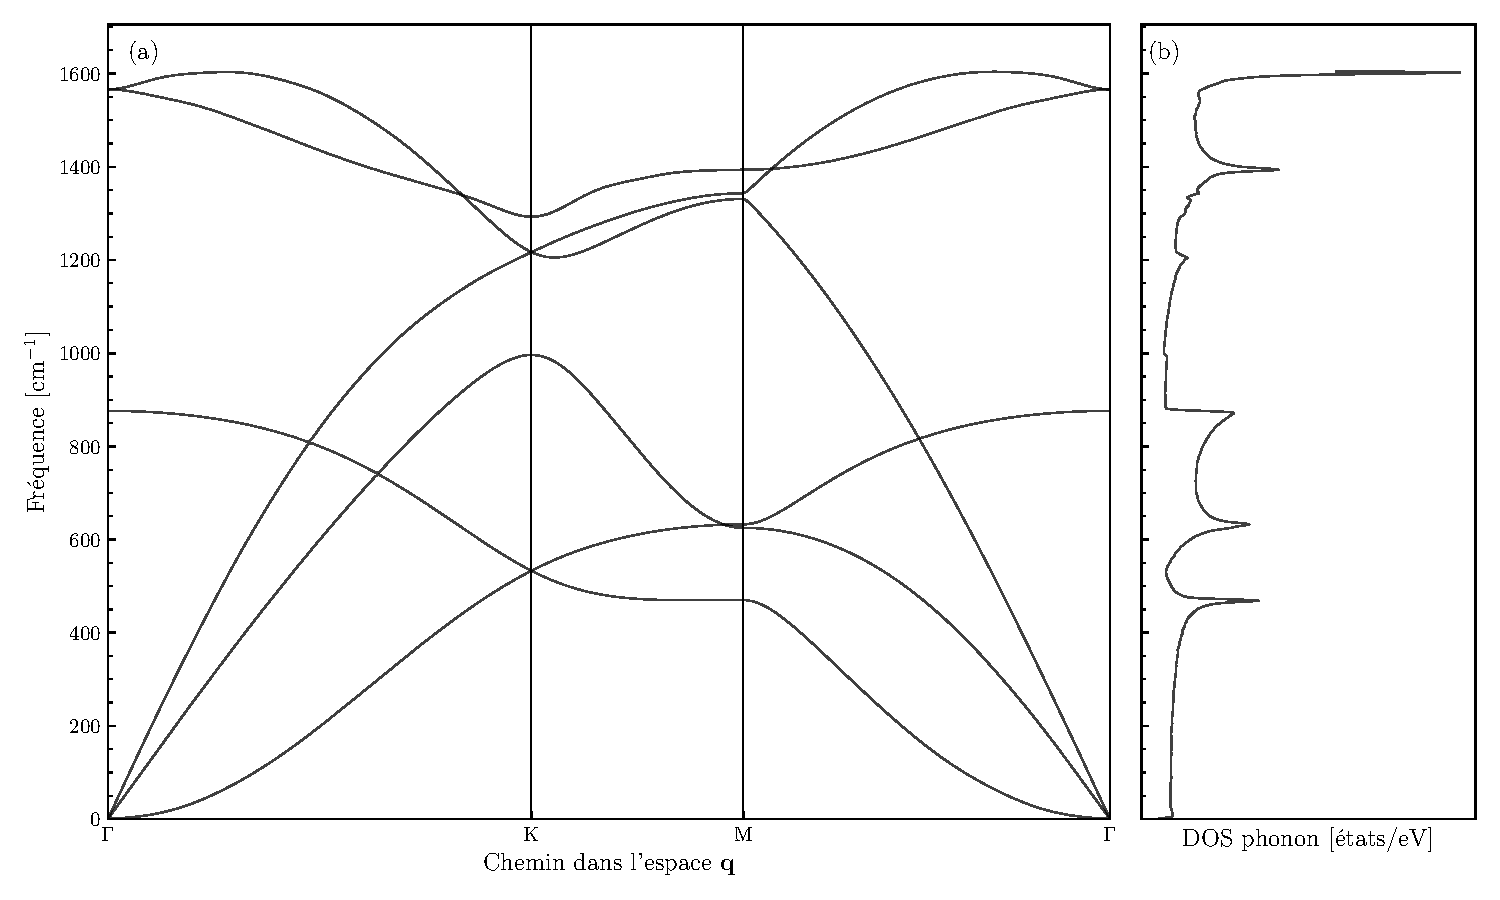
\includegraphics[width=\textwidth]{figures/fig_phonons.pdf}
    \caption[Fréquences et densité d'états des phonons pour une feuille de graphène parfaite.]{Fréquences et densité d'états des phonons pour une feuille de graphène parfaite. Les propriétés de l'état fondamental des électrons ont été obtenues sur une grille $\kv$ $32\times 32\times 1$, une coupure d'énergie cinétique de 100 Ry, un \textit{smearing} MV de 0.01 Ry, la fonctionnelle XC PBE, le pseudo-potentiel ONCV \textit{stringent} de PseudoDojo et un paramètre du réseau de $a=2.46$ \AA. Les propriétés de phonons ont été obtenues en résolvant les équations DFPT sur une grille $\qv$ $16\times 16\times 1$. (a) Fréquences des phonons obtenues sur le chemin de haute symétrie $\Gamma\to K\to M\to\Gamma$ 100 points par segment. (b) Densité d'états des phonons, calculée avec une grille $\qv$ $96\times96\times 1$ et un facteur d'élargissement de $\sigma=0.01$ Ry.} 
    \label{fig:phonon_results}
\end{figure}
Il est possible de définir la densité d'états des phonons d'une manière totalement analogue à la densité d'états électroniques:
\begin{equation}
    D(\omega)=\sum_{\nu\qv}\delta(\omega-\omega_{\nu\qv}).
\end{equation}
Comme pour la DOS électronique, numériquement il est nécessaire de remplacer la fonction delta par une Gaussienne avec un facteur d'élargissement $\sigma$.
Il faut un échantillonnage très dense de la BZ pour converger la DOS. À cet effet, nous utilisons une grille $\qv$ dense de $96\times 96\times 1$ et un facteur d'élargissement de $\sigma=0.01$ Ry pour calculer la DOS des phonons. Le résultat se trouve dans la figure~\ref{fig:phonon_results}--(b). La DOS présente plusieurs pics de Van Hove aux fréquences 
correspondant aux extrema des branches de phonons, notamment 
aux alentours de 500, 600, 900, 1400 et 1580~cm$^{-1}$, 
reflétant la structure de bande de phonons du panneau~(a).

\section{Fonctions de Wannier}
Tel que mentionné dans le chapitre~\ref{chap:Raman}, les équations d'intensité Raman sont particulièrement difficile à converger et requièrent des grilles $\kv$ et $\qv$ extrêmement denses~\cite{lazzeriFirstPrinciplesCalculationVibrational2003,gilletFirstprinciplesStudyExcitonic2013a,bagheriHighthroughputComputationRaman2023}. En pratique, obtenir les quantités électroniques avec la DFT et les quantités de phonons avec la DFPT sur des grilles aussi denses est computationnellement prohibitif. Pour contourner ce problème, nous pouvons interpoler les quantités obtenues par la DFT et la DFPT sur des grilles plus denses. Il existe plusieurs schémas d'interpolation : l'interpolation de Fourier~\cite{madsenBoltzTraP2ProgramInterpolating2018}, un calcul NSCF pour les quantités électroniques~\cite{bruninPhononlimitedElectronMobility2020}, le \textit{double padding}~\cite{bruninPhononlimitedElectronMobility2020}, le \textit{zero padding}, l'interpolation linéaire~\cite{liElectricalTransportLimited2015} et l'interpolation avec des fonctions de Wannier (WF)~\cite{ponceEPWElectronphononCoupling2016}. Nous utilisons cette dernière technique pour interpoler toutes les quantités nécessaires sur des grilles assez denses pour converger l'intensité Raman. 

Les WF offrent deux avantages considérables : une interpolation efficace qui permet l'interpolation sur des grilles ultra denses et la capacité de respecter la physique du système interpolé. Les WF fournissent une base localisée et cette localisation garantit que les éléments de matrice calculés dans cette base décroissent rapidement avec la distance, de sorte qu'une transformée de Fourier tronquée suffit pour reproduire fidèlement n'importe quelle propriété sur une grille arbitrairement dense et ce à faible coût numérique. De plus, la transformation vers les WF étant exacte et unitaire, les propriétés interpolées coïncident exactement avec les résultats \textit{ab initio} sur la grille originale. Ces aspects s'appliquent autant aux propriétés électroniques, aux propriétés vibrationnelles (phonons), aux propriétés des défauts et aux propriétés de couplage électron-phonon, faisant de l'interpolation de Wannier une technique efficace et générale. En plus de leur utilité pour l'interpolation, les fonctions de Wannier sont utilisées pour faire des modèle \textit{tight binding} effectif \textit{ab initio} qui servent d'entrée pour la DMFT~\cite{lechermannDynamicalMeanfieldTheory2006} et sont à la base de la théorie moderne de la polarisation~\cite{king-smithTheoryPolarizationCrystalline1993,restaMacroscopicPolarizationCrystalline1994}. Dans cette section, nous introduisons ce schéma d'interpolation.

\subsection{Définitions de base}
Les WF ont été introduites pour la première fois par
Wannier~\cite{wannierStructureElectronicExcitation1937} pour étudier
les niveaux d'excitation d'un électron dans un cristal. Tout comme
les fonctions de Bloch $\ket{\psi_{n\kv}}$, les WF forment une base
complète pour décrire les électrons dans un solide périodique.  Nous considérons
un sous-espace de $J$ bandes parmi les $N_b$ bandes calculées par
la DFT, pouvant contenir des dégénérescences et des croisements.
Une WF pour l'état $n$ localisée dans la cellule unitaire identifiée
par le vecteur du réseau $\Rv$ est dénotée $\ket{\Rv n}$ et est
définie par
\begin{equation}
    \ket{\Rv n} = \frac{1}{N_\kv}\sum_\kv e^{-i\kv\cdot\Rv}
    \sum_{m=1}^{N_b} U_{mn}^{(\kv)}\ket{\psi_{m\kv}},
    \label{eqn:c3_wf_1W}
\end{equation}
où $U^{(\kv)}$ est une matrice $N_b\times J$ à colonnes orthonormées,
périodique dans l'espace réciproque, et $N_\kv$ est le nombre de
points $\kv$ dans la grille \textit{ab initio}. La transformation
inverse reconstruit la projection des états de Bloch sur le
sous-espace des $J$ WF
\begin{equation}
    \ket{\tilde{\psi}_{n\kv}}=\sum_\Rv e^{i\kv\cdot\Rv}
    \sum_{m=1}^{J} U_{mn}^{(\kv)\dag}\ket{\Rv m}.
    \label{eqn:c3_wf_1B}
\end{equation}
Notons que l'information contenue dans les $N_b - J$ bandes exclues est
perdue. Les WF ne sont pas uniques puisque $U^{(\kv)}$ constitue un degré
de liberté arbitraire --- différents choix produisent des WF
physiquement équivalentes, mais avec des degrés de localisation
très différents. Pour que l'interpolation de Wannier soit aussi efficace que possible, nous cherchons les WF les plus localisées possible. Marzari et Vanderbilt~\cite{marzariMaximallyLocalizedGeneralized1997} proposent de fixer $U^{(\kv)}$ en minimisant la fonctionnelle de \textit{spread}
\begin{equation}
    \Omega = \sum_n\left[\langle \hat{r}^2\rangle_n - \langle \hat{\rv} \rangle^2_n\right],
\end{equation}
où 
\begin{equation}
    \langle \hat{r}^2\rangle_n = \bra{\mathbf{0}n}\hat{r}^2\ket{\mathbf{0}n},\qquad\langle \hat{\rv} \rangle_n = \bra{\mathbf{0}n}\hat{\rv}\ket{\mathbf{0}n},
\end{equation}
sont respectivement la dispersion quadratique moyenne et le centre de la WF $\ket{\mathbf{0}n}$. Les WF obtenues par cette minimisation sont appelées les fonctions de Wannier maximalement localisées (MLWF) et constituent le standard utilisé dans les schémas d'interpolation avec des fonctions de Wannier. Dans la prochaine section, nous voyons comment calculer les MLWF à partir des fonctions de Bloch $\ket{\psi_{n\kv}}$.

\subsection{Calculs des fonctions de Wannier}
Continuons avec le cas où nous considérons un sous-ensemble de $J$ bandes isolées de toutes les autres bandes. Il est utile de décomposer le \textit{spread} en deux contributions~\cite{marzariMaximallyLocalizedGeneralized1997}
\begin{equation}
    \Omega = \Omega_I + \widetilde{\Omega},
\end{equation}
où
\begin{equation}
    \Omega_I = \sum_n \left[ \bra{\mathbf{0}n}\hat{r}^2\ket{\mathbf{0}n} - 
    \sum_{\Rv m}\left|\bra{\Rv m}\hat{\rv}\ket{\mathbf{0}n}\right|^2 \right]
\end{equation}
est invariant sous toute transformation de jauge $U^{(\kv)}$, et
\begin{equation}
    \widetilde{\Omega} = \sum_n \sum_{\Rv m \neq \mathbf{0}n}
    \left|\bra{\Rv m}\hat{\rv}\ket{\mathbf{0}n}\right|^2
\end{equation}
est la partie dépendante de la jauge. Puisque $\Omega_I$ est fixe, minimiser le \textit{spread} $\Omega$ revient à minimiser $\widetilde{\Omega}$ uniquement. Pour l'évaluer explicitement, nous devons représenter l'opérateur position dans l'espace réciproque par différences finies sur la grille $\kv$. À cet effet, nous introduisons la matrice de recouvrement entre les états de Bloch voisins sur la grille 
\begin{equation}
    M^{(\kv,\bv)}_{mn}=\bra{u_{m\kv}}\ket{u_{n\kv+\bv}},
\end{equation}
où $\bv$ sont les vecteurs connectant chaque point $\kv$ à ses voisins sur la grille et $u_{n\kv}$ est la partie périodique de la fonction de Bloch. Cette matrice est l'objet central de la minimisation, car elle encode la variation des états de Bloch dans l'espace réciproque et est directement reliée à l'opérateur position. En effet, en utilisant la définition de la matrice $M^{(\kv,\bv)}$, il est possible de montrer que le centre et la dispersion quadratique moyenne de la WF $\ket{\mathbf{0}n}$ s'expriment comme
\begin{align}
    \langle \hat{\rv}\rangle_n &= -\frac{1}{N_\kv}\sum_{\kv\bv}w_\bv\bv\Im\log M_{nn}^{\kv,\bv},\label{eqn:c3_rn}\\
    \langle \hat{r}^2\rangle_n &= \frac{1}{N_\kv}\sum_{\kv\bv}w_\bv\left[\left(1-|M_{nn}^{\kv,\bv}|^2\right)+\left(\Im\log M_{nn}^{\kv,\bv}\right)^2\right],
\end{align}
où $w_\bv$ sont des poids qui dépendent du nombre de voisins et de la géométrie de la grille. Il s'ensuit que $\widetilde{\Omega}$ s'exprime entièrement en fonction de la matrice $M^{\kv,\bv}$ 
\begin{equation}
    \widetilde{\Omega}=\frac{1}{N_\kv}\sum_{\kv\bv}w_\bv\sum_{m\neq n}|M_{mn}^{\kv,\bv}|^2+\frac{1}{N_\kv}\sum_{\kv\bv}w_\bv\sum_n\left(-\Im\log M_{nn}^{\kv,\bv}-\bv\cdot\langle \hat{\rv}\rangle_n\right),
    \label{eqn:c3_omega_tilde}
\end{equation}
où $\langle\hat{\rv}\rangle_n$ est donné en termes de $M^{(\kv,\bv)}$ par l'équation~\eqref{eqn:c3_rn}. Ainsi, une fois que la matrice $M^{\kv,\bv}$ est calculée par le code DFT, aucune autre interaction avec les fonctions de Bloch n'est nécessaire. La minimisation de $\widetilde{\Omega}$ est effectuée par une descente de gradient dans l'espace des matrices. Le gradient de $\widetilde{\Omega}$ par rapport à $U^{(\kv)}$ est calculé analytiquement en fonction de $M^{(\kv,\bv)}$. Pour que la matrice $U^{(\kv)}$ garde ses propriétés au long de la minimisation, nous prenons la partie anti-hermitienne du gradient
\begin{equation}
    \mathcal{A}^{(\kv)}=\frac{1}{2}\left(\frac{\partial \widetilde{\Omega}}{\partial U^{(\kv)}}-\left(\frac{\partial \widetilde{\Omega}}{\partial U^{(\kv)}}\right)^\dag\right),
\end{equation}
qui définit la direction de descente. La mise à jour de $U^{(\kv)}$ est alors
\begin{equation}
   U^{(\kv)}\rightarrow U^{(\kv)}e^{\alpha \mathcal{A}^{(\kv)}},
\end{equation}
où $\alpha$ est le pas de descente. La matrice $M^{(\kv,\bv)}$ est mise à jour avec la nouvelle matrice $U^{(\kv)}$
\begin{equation}
    M^{(\kv,\bv)}\rightarrow U^{(\kv)\dag} M^{(\kv,\bv)}U^{(\kv+\bv)},
\end{equation}
et $\widetilde{\Omega}$ est mise à jour avec l'équation~\eqref{eqn:c3_omega_tilde}. Le processus est répété jusqu'à la convergence de $\widetilde{\Omega}$, produisant les MLWF. Cette minimisation est une procédure fortement non linéaire avec plusieurs minima locaux. Pour s'assurer de ne pas tomber sur un minimum local non physique, il est important de choisir une initialisation qui reflète la physique du système. À cet effet, un choix judicieux de point de départ est de projeter les fonctions de Bloch sur un ensemble de fonctions d'essai localisées $g_n(\rv)$, typiquement des orbitales atomiques ou des harmoniques sphériques centrées sur les sites atomiques. Cela est encodé dans la matrice de projection
\begin{equation}
    A^{(\kv)}_{mn} = \bra{\psi_{m\kv}}\ket{g_n}.
\end{equation}
La matrice initiale $U^{(\kv)}$ est obtenue par décomposition en valeurs singulières (SVD) de $A^{(\kv)}$. Ce choix garantit que la matrice initiale est le plus proche possible des projections physiques, ce qui stabilise la convergence des MLWF. Le choix des fonctions d'essai $g_n$ requiert une connaissance \textit{a priori} de la physique du système. Par exemple, pour étudier les électrons de valence dans un métal de transition, un bon choix d'essai serait les orbitales atomiques $d$. Pour un système avec une géométrie tétraédrique, des fonctions d'essai de type $sp^3$ sont un bon choix. Pour le graphène, si nous voulons avoir les MLWF pour les 3 plus basses bandes de valence ($\sigma$), il faut des fonctions d'essai de type $sp^2$. Pour la plus haute bande de valence ($\pi$) et la plus basse bande de conduction ($\pi^*$), il faut des orbitales $p_z$. 

\noindent\textbf{Bandes enchevêtrées}

Dans le cas d'un métal ou d'un semimétal, les bandes d'intérêt (proche du niveau de Fermi) croisent d'autres bandes et il est impossible d'isoler proprement un sous-espace de $J$ bandes pour tous les $\kv$. Ceci est particulièrement important pour le graphène, car la bande de conduction au niveau de Fermi ($\pi^*$) est enchevêtrée avec plusieurs bandes de plus haute énergie qui ne nous intéressent pas (voir la structure de bande à la figure~\ref{fig:resultats_electrons}--(a)). Pour pallier ce problème, Souza, Marzari et Vanderbilt~\cite{souzaMaximallylocalizedWannierFunctions2001} ont généralisé la procédure au cas de bandes enchevêtrées en introduisant une étape préalable de \textit{disentanglement}.

L'idée est de sélectionner, parmi un ensemble de $J'>J$ bandes contenues dans une fenêtre d'énergie extérieure, un sous-espace lisse de dimension $J$ qui varie continûment avec $\kv$. Ce sous-espace est caractérisé par une matrice rectangulaire $U^{\text{dis},(\kv)}$ de dimension $N_b\times J$
\begin{equation}
    \ket{\tilde{\psi}_{n\kv}}=\sum_{m=1}^{N_b}U_{mn}^{\text{dis},(\kv)}\ket{\psi_{m\kv}}\qquad n=1,\dots,J.
\end{equation}
Contrairement au cas de bandes isolées où $\Omega_I$ est fixe, il dépend ici du choix du sous-espace et peut être minimisé. Le sous-espace optimal est obtenu en minimisant $\Omega_I$ par rapport à $U^{\text{dis},(\kv)}$ avec une procédure similaire à la minimisation de $\widetilde{\Omega}$ par rapport à $U^{(\kv)}$. En pratique, il est possible de spécifier une deuxième fenêtre, la fenêtre gelée, dans laquelle les bandes DFT sont reproduites exactement par les MLWF. Ces bandes sont incluses telles quelles dans le sous-espace optimal pour tous les $\kv$ et la minimisation de $\Omega_I$ ne porte que sur les états en dehors de la fenêtre gelée (mais toujours dans la fenêtre extérieure). La fenêtre gelée est particulièrement utile pour figer les bandes proche du niveau de Fermi, lesquelles nous voulons reproduire exactement. Une fois le sous-espace optimal extrait et $U^{\text{dis},(\kv)}$ trouvé, la matrice $U^{(\kv)}$ est calculée en minimisant $\widetilde{\Omega}$ dans ce sous-espace en suivant la procédure décrite plus haut. Cette fois-ci, la matrice $U^{(\kv)}$ est carrée de dimension $J\times J$. La matrice de transformation totale est le produit des deux matrices
\begin{equation}
    \tilde{U}^{(\kv)} = U^{\text{dis},(\kv)}U^{(\kv)},
\end{equation}
et est une matrice rectangulaire $N_b\times J$. Les MLWF avec la procédure de \textit{disentanglement} sont
\begin{equation}
    \ket{\Rv n}=\frac{1}{N_\kv}\sum_{\kv}e^{-i\kv\cdot\Rv}\sum_{m=1}^{N_b}\tilde{U}^{(\kv)}_{mn}\ket{\psi_{m\kv}}.\label{eqn:c3_mlwf}
\end{equation}

\subsection{Interpolation de Wannier}
Une fois les MLWF obtenues pour les bandes d'intérêt, il est possible d'interpoler les quantités calculées sur la grille \textit{ab initio} vers une grille arbitrairement dense. L'idée centrale est de transformer la quantité d'intérêt dans la base des MLWF, où cette quantité est localisée dans l'espace réel, puis de la transformer de retour dans l'espace réciproque sur la grille dense par transformée de Fourier. 
Nous utilisons cette méthode d'interpolation pour avoir toutes les quantités sur des grilles denses nécessaires à l'évaluation de l'intensité Raman résonnante. 

Commençons par le cas prototypique de l'Hamiltonien électronique pour l'interpolation des valeurs propres $\varepsilon_{n\kv}$. Lorsque le problème est résolu avec la DFT, nous avons l'Hamiltonien dans la base de Bloch sur une grille modérément dense $\kv_c$
\begin{equation}
    H_{mn}(\kv_c) = \bra{\psi_{m\kv_c}}\hat{H}_\text{KS}\ket{\psi_{n\kv_c}}.
\end{equation}
L'Hamiltonien est diagonal dans l'indice de bande dans cette base. Ensuite, nous transformons l'Hamiltonien dans la base des MLWF à l'aide des matrices $U^{(\kv_c)}$ (ou des matrices $\tilde{U}^{(\kv_c)}$ si des bandes sont enchevêtrées)
\begin{equation}
    H_{mn}(\Rv) = \frac{1}{N_{\kv_c}}\sum_{\kv_c}e^{-i\kv_c\cdot\Rv}\left[U^{\dag(\kv_c)}H(\kv_c)U^{(\kv_c)}\right]_{mn}.
\end{equation}
Ensuite, l'Hamiltonien est reconstruit dans l'espace réciproque sur une grille $\kv_f$ arbitraire via une transformée de Fourier discrète 
\begin{equation}
    H_{mn}(\kv_f) = \sum_\Rv e^{i\kv_f\cdot\Rv}H_{mn}(\Rv).
\end{equation}
Maintenant, l'Hamiltonien est une matrice $J\times J$ qui n'est pas nécessairement diagonale. Toute l'information sur les bandes exclues a été perdue. Pour obtenir les valeurs propres interpolées sur la grille dense, il suffit de diagonaliser la matrice $H_{mn}(\kv_f)$. En même temps, nous obtenons la matrice $V_{mn}^{(\kv_f)}$ de dimension $J\times J$ qui contient les vecteurs propres de $H_{mn}(\kv_f)$. Cette matrice est importante pour l'interpolation de tous les autres opérateurs autre que l'Hamiltonien. 

Pour un opérateur général $\hat{O}$ dont nous connaissons la représentation dans la base des fonctions de Bloch $O_{mn}(\kv_c)=\bra{\psi_{m\kv_c}}\hat{O}\ket{\psi_{n\kv_c}}$ sur une grille modérément dense, l'interpolation de Wannier suit une procédure similaire à celle pour l'Hamiltonien. Nous commençons par le transformer dans la base des MLWF
\begin{equation}
    O_{mn}(\Rv)=\frac{1}{N_{\kv_c}}\sum_{\kv_c} e^{-i\kv_c\cdot\Rv}\left[U^{\dag(\kv_c)}O(\kv_c)U^{(\kv_c)}\right]_{mn}.
\end{equation}
Ensuite, l'opérateur est reconstruit dans l'espace réciproque sur une grille $\kv_f$ arbitraire par l'inverse de la transformation 
\begin{equation}
    O_{mn}(\kv_f) = \sum_{\Rv}e^{i\kv_f\cdot\Rv}\left[V^{(\kv_f)}O(\Rv)V^{\dag (\kv_f)}\right]_{mn},
\end{equation}
\begin{figure}
    \centering
    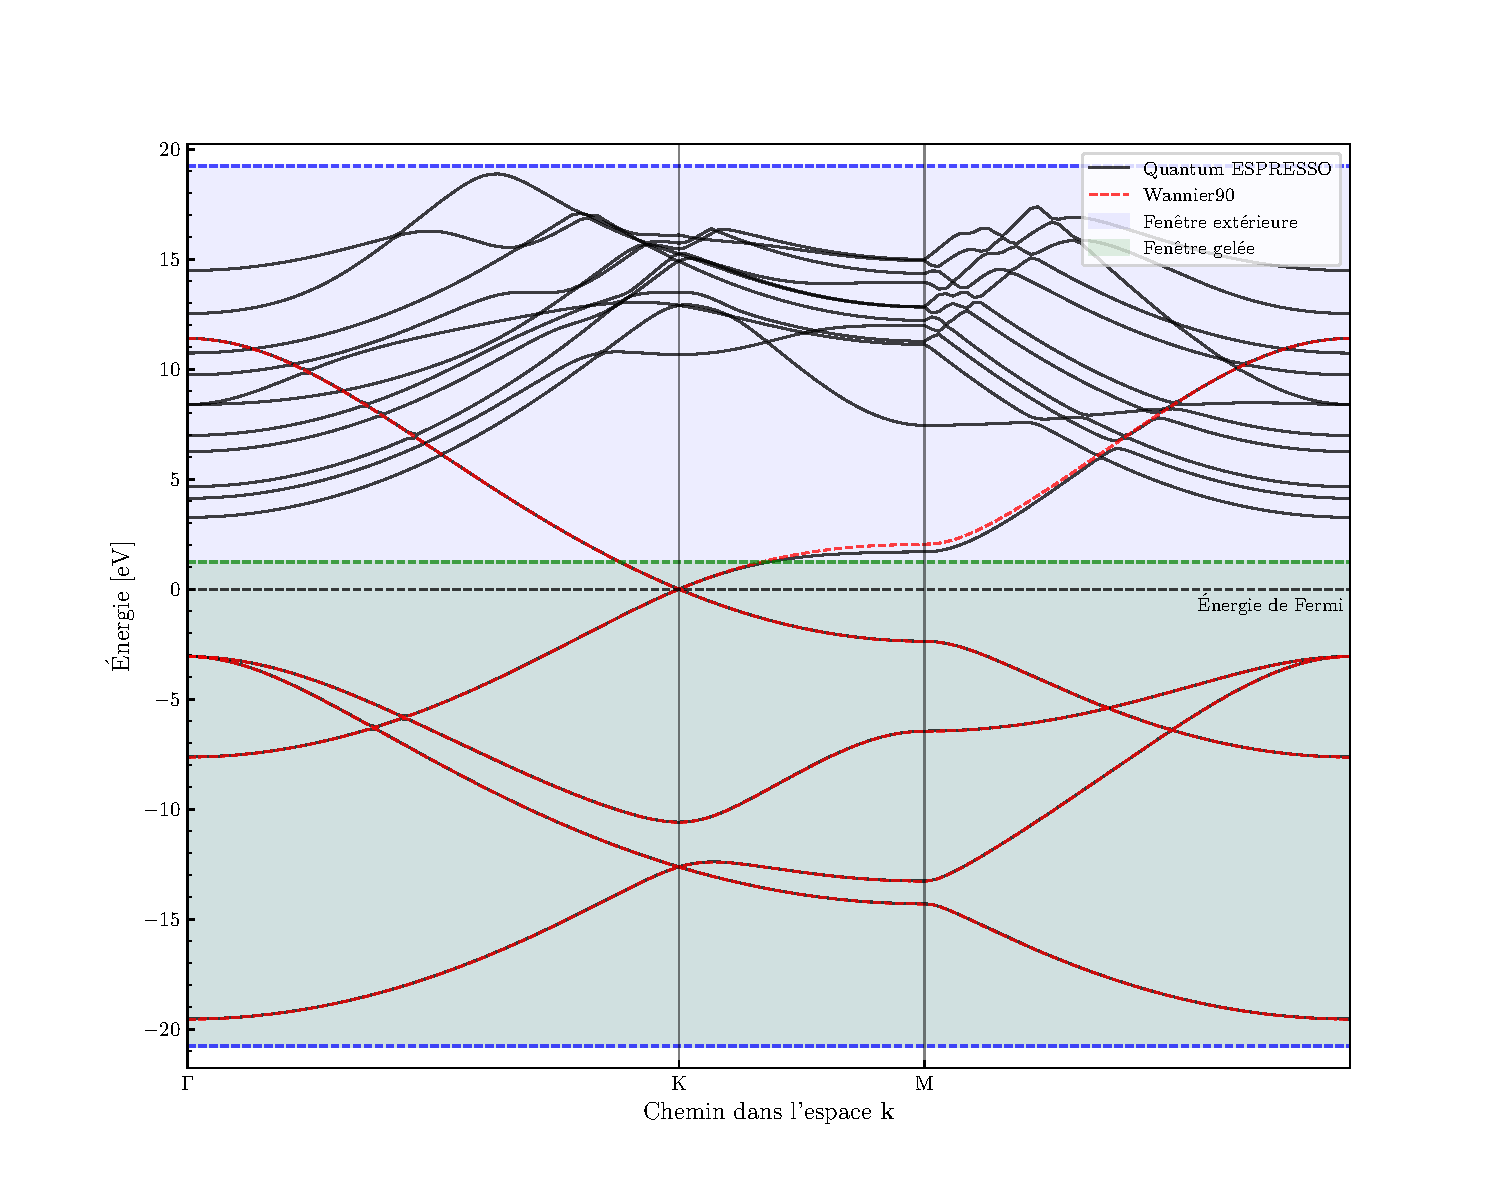
\includegraphics[width=\textwidth]{figures/fig_band_interp.pdf}
    \caption[Comparaison entre la structure de bandes DFT et l'interpolation de la structure de bandes du graphène parfait à l'aide des MLWF.]{Comparaison entre la structure de bandes DFT et l'interpolation de la structure de bandes du graphène parfait à l'aide des MLWF. La fenêtre gelée dans laquelle les bandes sont reproduites exactement en illustrée en vert. La fenêtre extérieure est représentée en bleu. Le calcul DFT de la structure de bandes à été calculée avec \texttt{Quantum ESPRESSO} avec les paramètres donnés à la section~\ref{sec:electron_results}. Les MLWF pour les 5 bandes de plus basse énergie pour le graphène ont été obtenues avec \texttt{Wannier90}.}
    \label{fig:band_interp}
\end{figure}
où $V^{(\kv_f)}$ est la matrice des vecteurs propres de l'Hamiltonien interpolé sur la grille dense. Notons que la multiplication par $V^{(\kv_f)}$ est nécessaire pour ramener les opérateurs dans la jauge de Bloch.  En effet, après une simple transformée de Fourier de $H_{mn}(\Rv)$ vers l'espace réciproque, l'Hamiltonien obtenu $H_{mn}(\kv_f)$ n'est pas diagonal, ce qui indique que nous ne sommes pas dans la jauge de Bloch. Pour y revenir, on diagonalise $H_{mn}(\kv_f)$, ce qui fournit les vecteurs propres $V^{(\kv_f)}$. Tout opérateur général $\hat{O}$ est ensuite ramené dans cette jauge via la transformation par $V^{(\kv_f)}$, comme indiqué dans l'équation ci-dessus. Si l'opérateur $O(\Rv)$ est bien localisé dans l'espace réel, \textit{i.e.} s'il décroît rapidement avec $|\Rv|$, la somme sur les vecteurs de réseau peut être tronquée après quelques termes, rendant l'interpolation extrêmement efficace même sur des grilles très denses.


Nous terminons cette section avec un exemple de l'interpolation de Wannier appliquée à l'Hamiltonien d'une feuille de graphène parfaite. L'Hamiltonien est diagonalisé sur la grille \textit{ab initio} modérément dense par un calcul SCF avec le code DFT \texttt{Quantum ESPRESSO} et les paramètres déterminés à la section~\ref{sec:electron_results}. Ensuite, les MLWF pour les 5 bandes les plus basses en énergie du graphène et l'Hamiltonien dans la base des MLWF sont calculées avec le logiciel \texttt{Wannier90}~\cite{mostofiWannier90ToolObtaining2008,mostofiUpdatedVersionWannier902014,pizziWannier90CommunityCode2020}. L'Hamiltonien est reconstruit et diagonalisé dans l'espace réciproque  sur le même chemin que la structure de bandes DFT pour comparer les deux. La comparaison est illustrée dans la figure~\ref{fig:band_interp}. Nous voyons que les bandes DFT sont exactement reproduites dans la fenêtre gelée (illustrée en vert). La fenêtre extérieure (en bleu) contient les bandes qui participent à l'extraction du sous-espace optimal de 5 bandes. 
Finalement, nous notons que \texttt{Wannier90} a besoin d'une grille $\kv$ uniforme, \textit{i.e.} qui n'est pas réduite par symétrie. La procédure habituelle est de faire le calcul SCF DFT sur la grille réduite par symétrie, puis de refaire un calcul NSCF, peu coûteux numériquement, sur une grille de même densité mais non réduite par symétrie.

\section{Photons}\label{sec:photon}
La spectroscopie Raman étant un processus de diffusion inélastique de la lumière, les photons y jouent un rôle central : un photon incident est absorbé par le système électronique, lequel émet un photon diffusé à une fréquence différente après avoir échangé de l'énergie avec un phonon. Ces processus de diffusions microscopiques requièrent une description quantique du champ électromagnétique, ainsi que l'expression du couplage entre les électrons et les photons, que nous introduisons brièvement dans cette section.

\subsection{Quantification du champ électromagnétique}
La quantification du champ électromagnétique suit la procédure standard de quantification canonique~\cite{hegerfeldtPhotonsAtomsIntroduction1990}. Dans la jauge de Coulomb ($\nabla\cdot\hat{\mathbf{A}}=0$), l'Hamiltonien du champ électromagnétique libre s'écrit
\begin{equation}
    \hat{H}_\text{em} = \sum_{\lambda\qv}\hbar\omega_{\qv}\left(\hat{a}_{\lambda\qv}^\dag\hat{a}_{\lambda\qv}+\frac{1}{2}\right),
\end{equation}
où $\hat{a}^\dag_{\lambda\qv}$ et $\hat{a}_{\lambda\qv}$ sont les opérateurs de création et d'annihilation d'un photon de vecteur d'onde $\qv$ et de polarisation $\lambda$, et $\omega_\qv=c|\qv|$ est la fréquence du photon ($c$ est la vitesse de la lumière). Les opérateurs de photons commutent entre eux $[\hat{a}_{\lambda\qv},\hat{a}_{\lambda'\qv'}]=[\hat{a}_{\lambda\qv}^\dag,\hat{a}^\dag_{\lambda'\qv'}] = 0$, ils sont donc des bosons. Le potentiel vecteur quantifié s'exprime en termes de ces opérateurs
\begin{equation}
    \hat{\mathbf{A}}(\rv)=\sum_{\lambda\qv}\sqrt{\frac{\hbar}{2\varepsilon_0\omega_\qv V}}\mathbf{e}_{\lambda\qv}\left(\hat{a}_{\lambda\qv}e^{i\qv\cdot\rv}+\hat{a}^\dag_{\lambda\qv}e^{-i\qv\cdot\rv}\right),
    \label{eqn:c3_A}
\end{equation}
où $\mathbf{e}_{\lambda\qv}$ est le vecteur de polarisation du photon $(\lambda\qv)$, $V$ est le volume du système et $\varepsilon_0$ est la permittivité du vide. 

\subsection{Couplage électron-photon}
Le champ électromagnétique couple avec les particules chargées d'un système, tels les électrons dans un solide. La prescription canonique est le couplage minimal qui revient à faire le remplacement $\hat{\mathbf{p}}\rightarrow \hat{\mathbf{p}}-e\hat{\mathbf{A}}$ dans l'Hamiltonien électronique. Cet ajout donne lieu à deux termes de couplage
\begin{equation}
    \hat{H}_\text{eem}=-\frac{e}{m_e}\hat{\mathbf{A}}\cdot\hat{\mathbf{p}}+\frac{e^2}{2m_e}\hat{\mathbf{A}}^2,
\end{equation}
où $e$ est la charge de l'électron et $m_e$ sa masse. Le deuxième terme, quadratique en $\hat{\mathbf{A}}$, est négligeable dans le régime des faibles intensités lumineuses et est souvent abandonné. De plus, en observant la forme du potentiel vecteur quantifié de l'équation~\eqref{eqn:c3_A}, nous voyons que ce terme est responsable des processus où il y a émission ou absorption de deux photons, ce qui ne se produit pas dans la diffusion Raman. Le premier terme, linéaire en $\hat{\mathbf{A}}$, est responsable de l'émission et l'absorption d'un photon et entre directement dans la diffusion Raman.

En ne gardant que ce premier terme et en l'écrivant en deuxième quantification, nous avons
\begin{equation}
    \hat{H}_\text{eem}=\sum_{mn\lambda}\sum_\kv g_{mn}^{(\lambda)}(\kv)\hat{c}^\dag_{m\kv}\hat{c}_{n\kv}(\hat{a}_\lambda+\hat{a}^\dag_\lambda)
\end{equation}
où nous avons défini les éléments de matrice de couplage électron-photon entre deux états de Bloch $\ket{\psi_{n\kv}}$ et $\ket{\psi_{m\kv}}$: 
\begin{equation}
    g^{(\lambda)}_{mn}(\kv) = -e\sqrt{\frac{\hbar}{2\varepsilon_0 \omega V}}\bra{\psi_{m\kv}}\mathbf{e}_\lambda\cdot\hat{\mathbf{v}}\ket{\psi_{n\kv}},
\end{equation}
et où nous avons supposé que le vecteur d'onde du photon est négligeable par rapport à celui de l'électron (c'est l'approximation dipolaire électrique) et nous avons réécrit l'opérateur impulsion en terme de l'opérateur de vitesse $\hat{\mathbf{p}}=m_e\hat{\mathbf{v}}$. En pratique, l'élément de matrice vitesse se calcule via l'Hamiltonien interpolé par les MLWF:
\begin{equation}
    v_{mn}(\kv)=\bra{\psi_{m\kv}}\hat{\mathbf{v}}\ket{\psi_{n\kv}}=\frac{1}{\hbar}\bra{\psi_{m\kv}}\nabla_\kv \hat{H}(\kv)\ket{\psi_{n\kv}} = \frac{1}{\hbar}\sum_{\Rv}e^{i\kv\cdot\Rv}i\Rv H_{mn}(\Rv),
\end{equation}
où dans la troisième égalité les fonctions de Bloch ont été écrites en termes des MLWF. La quantité $\Rv H_{mn}(\Rv)$ décroit rapidement avec $|\Rv|$ et les éléments de matrice de l'opérateur vitesse peuvent être calculés sur une grille très dense à faible coût computationnel. Finalement, pour avoir l'élément de matrice de couplage électron-photon, il faut faire la contraction de l'opérateur vitesse de l'électron avec le vecteur de polarisation du photon:
\begin{equation}
    g^{(\lambda)}_{mn}(\kv) = -e\sqrt{\frac{\hbar}{2\varepsilon_0\omega V}}\sum_\mu e_{\lambda\mu}v_{mn}^{(\mu)}(\kv),
\end{equation}
où $\mu=x,y,z$ identifie les coordonnées cartésiennes des vecteurs.

\section{Hamiltonien complet en deuxième quantification}
Avant de conclure ce chapitre, il vaut la peine de faire une petite pause pour récapituler le grand nombre de concepts théoriques qui ont été vus dans ce chapitre. Nous avons un système de graphène avec des défauts et trois types de particules élémentaires qui interagissent entre elles. L'Hamiltonien total de ce système se décompose en une partie libre et une partie d'interaction
\begin{equation}
    \hat{H} = \hat{H}_0+\hat{H}_\text{int}.
\end{equation}
La partie libre regroupe l'Hamiltonien électronique de KS diagonalisé et les Hamiltoniens libres phononique et photonique
\begin{equation}
    \hat{H}_0 =\underbrace{\sum_{n\kv}\varepsilon_{n\kv}\hat{c}^\dag_{n\kv}\hat{c}_{n\kv}}_{\hat{H}_\text{e}} + \underbrace{\sum_{\nu\qv}\hbar\omega_{\nu\qv}\left(\hat{b}^\dag_{\nu\qv}\hat{b}_{\nu\qv}+\frac{1}{2}\right)}_{\hat{H}_\text{ph}}+\underbrace{\sum_{\lambda\qv}\hbar\omega_{\lambda\qv}\left(\hat{a}_{\lambda\qv}^\dag \hat{a}_{\lambda\qv}+\frac{1}{2}\right)}_{\hat{H}_\text{em}}.
\end{equation}
Pour différencier entre les photons et les phonons: l'indice $\nu$ est associé aux quantités phononiques et l'indice $\lambda$ aux quantités photoniques. La partie d'interaction regroupe le couplage électron-photon, le couplage électron-défaut et le couplage électron-phonon
\begin{equation}
    \hat{H}_\text{int} = \underbrace{\sum_{mn\lambda}\sum_\kv g_{mn}^{(\lambda)}(\kv)\hat{c}^\dag_{m\kv}\hat{c}_{n\kv}(\hat{a}_\lambda+\hat{a}_\lambda^\dag)}_{\hat{H}_\text{eem}}+\hat{H}_\text{ed}+\hat{H}_\text{eph}.
\end{equation}
L'Hamiltonien de couplage électron-défaut $\hat{H}_\text{ed}$ est introduit dans le chapitre sur les défauts et l'Hamiltonien de couplage électron-phonon $\hat{H}_\text{eph}$ est introduit dans le chapitre sur le couplage électron-phonon, les chapitres~\ref{chap:défauts} et~\ref{chap:eph} respectivement, lesquels sont indispensables pour la diffusion Raman.

\section{Conclusion}
Pour conclure ce chapitre, nous avons obtenu les valeurs propres électroniques $\varepsilon_{n\kv}$ et les fonctions d'onde $\ket{\psi_{n\kv}}$ à l'aide de la DFT. Nous avons également utilisé les MLWF pour interpoler l'Hamiltonien électronique pour obtenir les valeurs propres $\varepsilon_{n\kv}$ sur une grille $\kv$ ultra dense à moindre coût computationnel. Nous avons également obtenu les fréquences de phonons $\omega_{\nu\qv}$ sur un grille modérément dense à l'aide de la DFPT. Nous les avons aussi obtenues sur une grille $\qv$ ultra dense grâce à une interpolation similaire à l'interpolation de Wannier pour les quantités électroniques. Finalement, nous avons introduit le couplage électron-photon et avons détaillé comment obtenir ces éléments de matrice sur une grille $\kv$ ultra dense dans l'approximation du dipôle électrique avec l'aide des MLWF. Dans les deux prochains chapitres, nous assemblons les dernières quantités requises pour l'évaluation de l'intensité Raman résonante du graphène avec des défauts, c'est-à-dire les quantités reliées au couplage électron-défaut et électron-phonon. 